\documentclass[11pt,a4paper]{article}

\usepackage[a4paper,margin=2cm]{geometry}
\usepackage[T1]{fontenc}
\usepackage{lmodern}
\usepackage{microtype}
\usepackage{amsmath}
\usepackage{amssymb}
\usepackage{amsthm}
\usepackage{graphicx}
\usepackage{booktabs}
\usepackage{xcolor}
\usepackage{caption}
\usepackage{hyperref}
\usepackage{listings}
\usepackage{tcolorbox}
\usepackage{algorithm}
\usepackage{algpseudocode}
\usepackage{enumitem}
\usepackage{titlesec}
\usepackage{array}

\hypersetup{
  colorlinks=true,
  linkcolor=blue!50!black,
  citecolor=blue!50!black,
  urlcolor=blue!50!black
}

% Compact section spacing -----------------------------------------------------
\titlespacing*{\section}{0pt}{1.6ex plus .3ex}{0.6ex}
\titlespacing*{\subsection}{0pt}{1.1ex plus .2ex}{0.4ex}
\titlespacing*{\subsubsection}{0pt}{0.8ex plus .2ex}{0.3ex}

% Numbered theorem-like environments ------------------------------------------
\theoremstyle{definition}
\newtheorem{example}{Example}[section]
\newtheorem{definition}{Definition}[section]

% A boxed call-out for intuition notes ----------------------------------------
\newtcolorbox{intuition}[1][]{%
  colback=blue!4,colframe=blue!40!black,
  fonttitle=\bfseries,
  title=Intuition,
  boxrule=0.5pt,
  arc=2pt,
  left=4pt,right=4pt,top=2pt,bottom=2pt,
  #1
}

% Listings setup --------------------------------------------------------------
\definecolor{codebg}{RGB}{246,246,248}
\definecolor{codecomment}{RGB}{120,120,120}
\definecolor{codekw}{RGB}{30,60,160}
\definecolor{codestr}{RGB}{40,140,40}
\lstdefinestyle{pystyle}{
  language=Python,
  backgroundcolor=\color{codebg},
  basicstyle=\ttfamily\small,
  keywordstyle=\color{codekw}\bfseries,
  commentstyle=\color{codecomment}\itshape,
  stringstyle=\color{codestr},
  numbers=none,
  showstringspaces=false,
  breaklines=true,
  frame=single,
  rulecolor=\color{black!15},
  framesep=4pt,
  xleftmargin=0pt,
  aboveskip=4pt,
  belowskip=4pt,
}
\lstset{style=pystyle}

% Caption styling -------------------------------------------------------------
\captionsetup{font=small,labelfont=bf,skip=3pt}

% Title -----------------------------------------------------------------------
\title{
  \vspace{-1em}
  \textbf{A Mathematical Tour of Lane Detection and\\
  Autonomous Steering Control} \\[0.3em]
  \large A pedagogical companion to the project for a CS student}
\author{David Tovmasyan \\
  \href{mailto:david.tovmasyan@connectto.com}{\texttt{david.tovmasyan@connectto.com}}}
\date{May 2026}

\begin{document}
\maketitle

\begin{abstract}
\noindent
This document is the long-form, mathematically explicit companion to
the project ``Real-Time Lane Detection and Autonomous Steering''.
Where the short report focused on the experimental story, this
document tells the \emph{pedagogical} story: every formula behind every
stage of every method is derived, illustrated with worked numerical
examples, and tied back to the actual lines of Python in the
repository. The reader is assumed to be a third-year CS student
comfortable with linear algebra and basic calculus, but not
necessarily familiar with computer vision or feedback control. By the
end of the document, you should be able to (a)~reimplement each
detector from scratch, (b)~explain why the proposed bird's-eye-view
polynomial-fit detector outperforms a Hough-line baseline on curved
tracks, and (c)~analyse a PID and a Stanley controller as feedback
laws on the bicycle model.
\end{abstract}

\vspace{0.5em}
{\small\tableofcontents}

\vspace{1em}

% ── Part 1: intro through the Hough detector ─────────────────────────
% =====================================================================
% Part 1: Introduction through the Hough detector (sections 1–6)
% Included by explanation.tex.
% =====================================================================

\section{Introduction and Motivation}
\label{sec:intro}

Lane keeping is, by a comfortable margin, the most widely deployed
function in modern advanced driver-assistance systems (ADAS). Every
mass-market car with ``lane-keep assist'' or ``lane-centering'' on its
spec sheet contains -- somewhere behind a windshield-mounted camera --
some version of the pipeline this document explains. The economics are
unromantic but compelling: a \$20 image sensor, a \$2 microcontroller,
and a few thousand lines of code can subtract the most common cause of
single-vehicle highway crashes (drift out of lane due to inattention or
drowsiness). For the same reason, lane detection has become a
near-universal entry point into autonomy: it is geometrically simple,
visually intuitive, and tractable on a CPU. It is therefore an ideal
classroom problem -- a tiny slice of self-driving that nevertheless
exercises camera calibration, image processing, edge detection, line
fitting, polynomial regression, vehicle dynamics, and feedback control.

\paragraph{The perception--planning--control split.}
Autonomous-driving stacks are almost always organised into three
layers, executed once per frame in a fixed pipeline:
\begin{enumerate}[leftmargin=2em,itemsep=2pt]
  \item \textbf{Perception} -- read the camera (and, in real cars,
        radar, LiDAR, IMU), and produce a structured description of the
        world: ``the left lane boundary is the curve $x = a y^2 + b y + c$''.
  \item \textbf{Planning} -- from that description, decide where the
        car should be in the next few hundred milliseconds: ``stay
        centred between the boundaries with a small look-ahead''.
  \item \textbf{Control} -- compute the steering and throttle commands
        that drive the vehicle toward that target, given the vehicle's
        current dynamic state.
\end{enumerate}
In this project the same split is visible: \texttt{lane\_methods.py}
implements perception, the lane-centre target is computed implicitly as
``the midpoint of the two boundary curves'', and \texttt{controller.py}
implements two control laws (PID and Stanley). The simulator -- the
\texttt{camera.py} renderer, the \texttt{track.py} spline and the
\texttt{vehicle.py} bicycle model -- replaces the physical world.

\paragraph{Why classical CV rather than deep learning?}
A naive reading of the recent literature might suggest the problem is
``solved'' by learning. State-of-the-art lane detectors -- LaneNet,
SCNN, PolyLaneNet, Ultra-Fast-Lane-Detection -- learn an end-to-end
map from pixels to lane parameters and dominate every public benchmark
(TuSimple, CULane, LLAMAS). Why then would anyone deploy a
hand-written Canny + Hough pipeline in 2026?
\begin{itemize}[leftmargin=1.4em,itemsep=2pt]
  \item \textbf{Interpretability.} Every step of the classical pipeline
        has a closed-form mathematical definition. If the car
        misbehaves, the failure can be traced to a specific stage: the
        ROI was wrong, the threshold was too high, the Hough binning
        was too coarse. With a black-box CNN this kind of forensic
        analysis is far harder.
  \item \textbf{Compute footprint.} The full pipeline in this project
        runs at $>1000$ FPS on a single CPU thread; a learned
        segmenter typically needs a GPU or NPU. For low-end ADAS
        modules without an accelerator, classical CV is the only
        option.
  \item \textbf{No training data, no labelling, no domain shift.}
        A classical detector contains no learned weights, so there is
        no train/test distribution mismatch. Its assumptions are
        visible (``edges of constant gradient form lines''), so we can
        predict \emph{a priori} where it will fail.
  \item \textbf{Educational clarity.} For a course project, every line
        of \texttt{HoughDetector.detect} is a piece of mathematics we
        can derive. Every line of a UNet is opaque.
\end{itemize}
The trade-off is equally clear: classical detectors assume a clean,
high-contrast world. They struggle with shadows, weathered paint,
crowded roads, and -- as we will see in detail -- with curves. The
question this project answers is therefore very specific: given that
the textbook Hough lane detector clearly fails on curves, how much of
that gap can be closed by a slightly less classical method that still
avoids deep learning? The proposed answer -- a bird's-eye
sliding-window quadratic fit -- reduces RMS lateral error by $34\%$ on
average across five tracks, while remaining interpretable and
real-time.

\paragraph{Roadmap of this document.}
This document is the long-form, pedagogical companion to the project.
The short report (\texttt{presentation/report.tex}) gives the
experimental punch line in three pages; this document gives every
derivation, every worked example, and every line of code behind the
punch line.
\begin{itemize}[leftmargin=1.4em,itemsep=2pt]
  \item Section~\ref{sec:prelim} covers the mathematical preliminaries:
        images as functions, colour spaces, convolution, Gaussian
        smoothing, the Sobel operator, and the four steps of the Canny
        edge detector. If you have not seen these before, this is
        where to spend the most time.
  \item Section~\ref{sec:sim} dissects the simulator: the
        Catmull--Rom spline that defines each track, the discrete
        curvature formula, the bicycle kinematic model, and the
        pinhole camera that produces the first-person image the
        detectors see.
  \item Section~\ref{sec:sub} formalises the lane-detection sub-problem:
        what the detectors are asked to compute, and what ground truth
        is available for evaluation.
  \item Section~\ref{sec:centroid} works through the first detector --
        the centroid baseline -- and explains, with image moments, why
        it cannot possibly succeed.
  \item Section~\ref{sec:hough} works through the second detector --
        the Hough-line pipeline -- in full mathematical detail,
        including the polar parameterisation of a line, the
        probabilistic Hough variant used by OpenCV, slope
        classification, length-weighted averaging, and temporal
        exponential smoothing.
\end{itemize}
The second half of the document (Part~2) picks up with the
inverse-perspective mapping and the proposed polynomial-fit detector,
then continues into vehicle control and the experimental evaluation.

% =====================================================================
\section{Mathematical Preliminaries}
\label{sec:prelim}

Before we can speak meaningfully about ``detecting lanes'' we need to
agree on what an image is, and on the handful of operations we will
perform on it. This section is deliberately slow: a third-year CS
student who has never taken a CV class should be able to follow every
formula and reproduce every numerical example by hand.

\subsection{An image is a function}

\begin{definition}[Discrete image]
A grayscale image of width $W$ and height $H$ is a function
\[
I : \{0,\ldots,W-1\}\times\{0,\ldots,H-1\}\to\{0,\ldots,255\},
\]
mapping integer pixel coordinates $(u,v)$ to an 8-bit intensity. A
colour image has the same domain but a three-component codomain,
$I:(u,v)\mapsto(R,G,B)\in\{0,\ldots,255\}^3$.
\end{definition}

Two conventions must be stated explicitly because they trip up almost
every newcomer:
\begin{enumerate}[leftmargin=2em,itemsep=2pt]
  \item The origin is at the \emph{top-left} of the image. The first
        axis $u$ increases to the right; the second axis $v$ increases
        downward. This is opposite to the convention you learned in
        calculus class, where $y$ usually points up.
  \item In our simulator the world coordinate $(X,Y)$ uses the same
        screen-down convention as the image (because everything is
        drawn into a Pygame window whose origin is also top-left). Be
        careful not to confuse image pixels and world pixels: the
        camera's $640\times480$ frame is one coordinate system; the
        $1400\times800$ Pygame window is another.
\end{enumerate}
The camera in this project produces images of size $W=640$, $H=480$
(set in \texttt{config.py}: \texttt{CAMERA\_IMG\_W=640},
\texttt{CAMERA\_IMG\_H=480}). A single frame is a NumPy array of shape
\texttt{(480, 640, 3)} with \texttt{dtype=uint8}.

\subsection{RGB to grayscale}

The first thing every classical detector in this project does is throw
away colour: it converts the RGB image to a single-channel grayscale
image. The standard conversion follows ITU-R Recommendation BT.601
(``Rec.~601''), originally designed so that the luminance channel of
analogue colour television matches what a human eye perceives as
brightness:
\begin{equation}
Y = 0.299\,R + 0.587\,G + 0.114\,B.
\label{eq:gray}
\end{equation}
The coefficients are not arbitrary: the human eye is much more
sensitive to green than to red, and least sensitive to blue. A simple
unweighted average $(R+G+B)/3$ would make red and green grass look
almost identical even though they are visually obviously different.

\begin{example}[Grayscale of a road pixel]
Our simulator paints the road in $\text{RGB}=(64,68,74)$ (see
\texttt{config.py:ROAD\_SURFACE}). Applying \eqref{eq:gray}:
\[
Y = 0.299\cdot 64 + 0.587\cdot 68 + 0.114\cdot 74
  \approx 19.14 + 39.92 + 8.44 \approx 67.5.
\]
So the road has roughly intensity 68 on a $[0,255]$ scale -- a fairly
dark grey, but well above black. Compare to grass
$\text{RGB}=(34,52,30)$: $Y\approx 10.2+30.5+3.4 = 44.1$. The road is
about $50\%$ brighter than the grass; that contrast is what lets the
Canny edge detector discover the road boundary.
\end{example}

In OpenCV the call is \texttt{cv2.cvtColor(img, cv2.COLOR\_RGB2GRAY)}
and it is the very first line of every \texttt{detect()} method in
this project (e.g.\ \texttt{lane\_methods.py:HoughDetector.detect},
line~203).

\subsection{The HSV colour space}

Sometimes we want to threshold by colour rather than brightness -- for
example, to find the yellow centre dashes
(\texttt{LANE\_DASH\_COLOR}\,=\,(200,200,80)) regardless of how
brightly lit they are. RGB is awkward for this because ``yellow'' is
a curve in 3-space rather than an axis; HSV separates the perceptual
axes:
\begin{itemize}[leftmargin=1.4em,itemsep=2pt]
  \item \textbf{Hue} $H\in[0,360^\circ)$: which colour. Red $\approx 0$,
        yellow $\approx 60$, green $\approx 120$, cyan $\approx 180$,
        blue $\approx 240$, magenta $\approx 300$. (OpenCV stores $H$
        scaled to $[0,180)$ so it fits in a \texttt{uint8}.)
  \item \textbf{Saturation} $S\in[0,1]$: how colourful. $S=0$ is pure
        grey; $S=1$ is fully saturated.
  \item \textbf{Value} $V\in[0,1]$: how bright. $V=0$ is black; $V=1$
        is the brightest version of the hue.
\end{itemize}
The conversion is piecewise. Given $R,G,B\in[0,1]$, let
$M=\max(R,G,B)$, $m=\min(R,G,B)$ and $C=M-m$. Then $V=M$, $S=C/M$ (if
$M>0$, else $0$), and
\[
H = 60^\circ\cdot
\begin{cases}
   \dfrac{G-B}{C}\bmod 6, & M=R,\\[4pt]
   \dfrac{B-R}{C} + 2,    & M=G,\\[4pt]
   \dfrac{R-G}{C} + 4,    & M=B.
\end{cases}
\]

\begin{example}[HSV of the road pixel]
Take the road colour $(R,G,B)=(64,68,74)$. Normalise to $[0,1]$:
$(0.251,0.267,0.290)$. Then $M=0.290$ (the blue channel), $m=0.251$,
$C=0.039$.
\begin{align*}
V &= 0.290 \;\Rightarrow\; V\cdot 255 \approx 74,\\
S &= C/M = 0.039/0.290 \approx 0.135 \;\Rightarrow\; S\cdot 255 \approx 34,\\
H &= 60^\circ\!\left(\tfrac{R-G}{C}+4\right)
   = 60^\circ\!\left(\tfrac{-0.016}{0.039}+4\right)
   \approx 60^\circ\cdot 3.59 \approx 215^\circ.
\end{align*}
So the road sits at hue $\approx 215^\circ$ (a slightly cool
blue-grey, which is correct -- the colour is barely off neutral), low
saturation $\approx 34/255$, and moderate value $\approx 74/255$. The
\texttt{CentroidDetector} uses precisely this signature to threshold
the road: \texttt{(s<40) \& (v>40) \& (v<110)} (line~122 of
\texttt{lane\_methods.py}). The chosen bounds bracket exactly the
$(S,V)$ values we just computed.
\end{example}

\subsection{2D convolution}

Everything we do to the image after grayscale conversion -- blurring,
edge detection, gradient estimation -- is a linear filter, and every
linear filter can be written as a convolution between the image $I$
and a small kernel $K$.

\begin{definition}[2D discrete convolution]
Given image $I$ and kernel $K$ of size $(2k{+}1)\times(2k{+}1)$, the
convolution $(I*K):\mathbb{Z}^2\to\mathbb{R}$ is
\begin{equation}
(I*K)(u,v) = \sum_{i=-k}^{k}\sum_{j=-k}^{k}
            I(u-i,v-j)\,K(i,j).
\label{eq:conv}
\end{equation}
\end{definition}

The minus signs in \eqref{eq:conv} are not a typo: a true convolution
flips the kernel before sliding it. In practice many image-processing
libraries (OpenCV included) actually compute the \emph{correlation}
$(I\star K)(u,v) = \sum_{i,j} I(u+i,v+j)K(i,j)$ -- with no flip -- and
call it convolution. For symmetric kernels (Gaussian, mean,
Sobel-magnitude\footnote{Sobel $S_x$, $S_y$ are antisymmetric, but the
sign convention is folded into the definition; what matters is being
consistent.}) the two operations agree, so the pedantry rarely bites.

\begin{example}[A $3\times 3$ box blur]
Consider a tiny grayscale image and a $3\times 3$ averaging kernel:
\[
I = \begin{pmatrix}10 & 20 & 30 \\ 40 & 50 & 60 \\ 70 & 80 & 90\end{pmatrix},\quad
K = \frac{1}{9}\begin{pmatrix}1&1&1\\1&1&1\\1&1&1\end{pmatrix}.
\]
At the centre pixel $(1,1)$ the convolution is the mean of all nine
values, $(10+20+\cdots+90)/9 = 450/9 = 50$. So $(I*K)(1,1)=50$. At a
boundary pixel we have to decide how to handle the missing neighbours;
OpenCV by default replicates the edge value, but the convolution
formula is identical otherwise.
\end{example}

\subsection{The Gaussian kernel}

Random pixel noise (and noise added in our experiments via
\texttt{evaluate.py:\_add\_noise}) is the enemy of edge detection: a
single bright spike inside an otherwise smooth patch produces a strong
gradient that no edge actually exists. The standard remedy is to blur
the image with a Gaussian kernel before computing gradients:
\begin{equation}
G_\sigma(x,y) = \frac{1}{2\pi\sigma^2}\exp\!\left(-\frac{x^2+y^2}{2\sigma^2}\right).
\label{eq:gauss}
\end{equation}
The function is rotationally symmetric and integrates to $1$ over
$\mathbb{R}^2$; in discrete form we sample \eqref{eq:gauss} at integer
offsets, then renormalise so the sampled values sum exactly to $1$ (to
preserve average brightness).

\begin{example}[$5\times 5$ Gaussian with $\sigma=1$]
Sampling \eqref{eq:gauss} at $(x,y)\in\{-2,-1,0,1,2\}^2$ with
$\sigma=1$ gives the unnormalised values
\[
\tilde G=\begin{pmatrix}
0.0030 & 0.0133 & 0.0219 & 0.0133 & 0.0030\\
0.0133 & 0.0596 & 0.0983 & 0.0596 & 0.0133\\
0.0219 & 0.0983 & 0.1620 & 0.0983 & 0.0219\\
0.0133 & 0.0596 & 0.0983 & 0.0596 & 0.0133\\
0.0030 & 0.0133 & 0.0219 & 0.0133 & 0.0030
\end{pmatrix}.
\]
The entries sum to about $0.9989$, so renormalising hardly changes
them. A common integer approximation (used in many introductory
tutorials) is
\[
G = \frac{1}{273}\begin{pmatrix}
1 & 4 & 7 & 4 & 1\\
4 & 16 & 26 & 16 & 4\\
7 & 26 & 41 & 26 & 7\\
4 & 16 & 26 & 16 & 4\\
1 & 4 & 7 & 4 & 1
\end{pmatrix},
\]
whose centre value $41/273\approx 0.150$ is close to the exact
$0.162$. Our project calls
\texttt{cv2.GaussianBlur(gray, (5,5), 0)} (line~204 of
\texttt{lane\_methods.py}); passing $\sigma=0$ tells OpenCV to derive
$\sigma$ from the kernel size as
$\sigma = 0.3((k-1)/2-1)+0.8\approx 1.1$, which is essentially the
kernel we just built.
\end{example}

A larger $\sigma$ blurs more aggressively, removes finer noise, but
also smears out genuine edges. The $5\times 5$ kernel with
$\sigma\approx 1$ is a good default for $640\times 480$ images: it
attenuates pixel-scale noise without dissolving lane markings.

\subsection{Image gradients: the Sobel operator}

An edge is, intuitively, a place where the image brightness changes
rapidly. Mathematically: a place where the spatial derivative
$\nabla I$ has a large magnitude. To approximate $\nabla I$ on a
discrete grid we convolve with the Sobel kernels:
\begin{equation}
S_x = \begin{pmatrix}-1 & 0 & 1\\-2 & 0 & 2\\-1 & 0 & 1\end{pmatrix},\quad
S_y = \begin{pmatrix}-1 & -2 & -1\\ 0 & 0 & 0\\ 1 & 2 & 1\end{pmatrix}.
\label{eq:sobel}
\end{equation}
Each kernel is the discrete tensor product of a smoothing kernel
$(1,2,1)$ in one direction with a central-difference derivative
$(-1,0,1)$ in the other; you can think of $S_x$ as ``smooth vertically
then differentiate horizontally''. The output channels $G_x=I*S_x$ and
$G_y=I*S_y$ are the estimated partial derivatives; gradient magnitude
and direction follow:
\begin{equation}
|G| = \sqrt{G_x^2+G_y^2},\qquad
\alpha = \operatorname{atan2}(G_y,G_x).
\label{eq:grad}
\end{equation}
The \texttt{PolyFitDetector} uses $S_x$ explicitly to find
vertical-ish lane markings (line~406 of \texttt{lane\_methods.py}:
\texttt{cv2.Sobel(gray, cv2.CV\_32F, 1, 0, ksize=3)}). The Hough
detector does not call Sobel directly because the Canny edge detector
(below) does it internally.

\subsection{Canny edge detection}

\texttt{cv2.Canny} reduces a grayscale image to a binary edge map:
pixel $(u,v)$ is $255$ if Canny believes there is an edge there, and
$0$ otherwise. The Canny algorithm (Canny 1986) is composed of four
steps that are all worth understanding individually:
\begin{enumerate}[leftmargin=1.6em,itemsep=2pt]
  \item \textbf{Gaussian blur.} As described above, smooth the image
        to suppress single-pixel noise. Without this step the
        derivatives in step~2 would amplify every speckle.
  \item \textbf{Sobel gradients.} Compute $G_x,G_y$ and the gradient
        magnitude $|G|$ from \eqref{eq:grad}. The magnitude image
        already looks like an edge map -- but it is too thick (real
        edges are typically several pixels wide because the gradient
        is non-zero across the whole transition), and includes weak
        responses everywhere.
  \item \textbf{Non-maximum suppression.} For each pixel, check
        whether its gradient magnitude is larger than that of its two
        immediate neighbours along the gradient direction $\alpha$. If
        not, zero it out. This thins the edge map to single-pixel-wide
        ridges, which is what we need for line fitting.
  \item \textbf{Double-threshold hysteresis.} A high threshold $T_H$
        marks ``strong'' edges; a low threshold $T_L$ marks
        ``candidate'' edges. A candidate edge is retained iff it is
        connected (8-neighbourhood) to a strong edge. This hysteresis
        is what makes Canny robust: an edge that peaks weakly but is
        part of a long contour survives, while isolated weak edges
        (noise) are discarded.
\end{enumerate}
This project uses \texttt{cv2.Canny(blurred, 50, 150)} with
$T_L=50$, $T_H=150$ (\texttt{config.py:CANNY\_LOW=50},
\texttt{CANNY\_HIGH=150}). The classical heuristic is $T_H:T_L$
between $2{:}1$ and $3{:}1$; we use exactly $3{:}1$. These specific
numbers were tuned against the simulator's road colours: $50$ is just
above the noise floor of the rendered frame, and $150$ comfortably
excludes everything except the sharp lane-boundary edges.

\begin{intuition}
An edge is where the image brightness changes fast in some direction.
Canny finds those places, thins the response so each edge is exactly
one pixel wide, and then keeps only the ones long enough (via
hysteresis) to be a real contour rather than a stray noise spike.
Everything else in the lane-detection pipeline operates on this
thinned binary picture.
\end{intuition}

% =====================================================================
\section{The Driving Simulator}
\label{sec:sim}

The simulator is small but it is doing a surprising amount of work:
generating a smooth closed-loop track, computing its curvature,
simulating a kinematic bicycle vehicle, and rendering the world
through a virtual pinhole camera. We treat each piece in turn.

\subsection{Track geometry: the Catmull--Rom spline}

A track in \texttt{config.py} is a list of $n$ waypoints
$\mathbf{p}_0,\mathbf{p}_1,\ldots,\mathbf{p}_{n-1}\in\mathbb{R}^2$
(e.g.\ 12 for the oval, 21 for Red Bull Ring). Connecting them with
straight line segments would give a polygon, not a track -- the
resulting heading changes would be discontinuous, the steering would
saturate at every waypoint, and the simulation would look terrible. We
need a smooth curve that passes through every waypoint.

\begin{definition}[Catmull--Rom spline]
Given four control points $\mathbf{p}_0,\mathbf{p}_1,\mathbf{p}_2,\mathbf{p}_3$,
the Catmull--Rom spline segment between $\mathbf{p}_1$ and
$\mathbf{p}_2$ is
\begin{equation}
\mathbf{q}(t)=\tfrac{1}{2}\Big[
  (2\mathbf{p}_1)
  + (-\mathbf{p}_0+\mathbf{p}_2)\,t
  + (2\mathbf{p}_0-5\mathbf{p}_1+4\mathbf{p}_2-\mathbf{p}_3)\,t^2
  + (-\mathbf{p}_0+3\mathbf{p}_1-3\mathbf{p}_2+\mathbf{p}_3)\,t^3
\Big],
\label{eq:catmull}
\end{equation}
for $t\in[0,1]$. The spline passes through $\mathbf{p}_1$ at $t=0$ and
$\mathbf{p}_2$ at $t=1$, while $\mathbf{p}_0$ and $\mathbf{p}_3$ control
the tangents at the endpoints.
\end{definition}

To check the interpolation property, substitute $t=0$ into
\eqref{eq:catmull}: the $t^1,t^2,t^3$ terms vanish, leaving
$\mathbf{q}(0)=\tfrac{1}{2}\cdot 2\mathbf{p}_1 = \mathbf{p}_1$.
Likewise $t=1$ gives $\mathbf{q}(1)=\mathbf{p}_2$. Differentiating,
\[
\mathbf{q}'(0)=\tfrac{1}{2}(\mathbf{p}_2-\mathbf{p}_0),\qquad
\mathbf{q}'(1)=\tfrac{1}{2}(\mathbf{p}_3-\mathbf{p}_1),
\]
so the tangent at $\mathbf{p}_1$ is parallel to the chord
$\mathbf{p}_2-\mathbf{p}_0$ -- the segment ``aims through'' the next
waypoint. The same tangent value is shared by the adjacent segment, so
the assembled curve is $C^1$-continuous (no kinks in heading) through
every waypoint. That is exactly what a drivable track needs.

In code (\texttt{track.py:Track.\_interpolate}, lines~31--52), the
spline is sampled at \texttt{TRACK\_SAMPLES\_PER\_SEGMENT~=~60} values
of $t\in[0,1)$ per segment, looping the index modulo $n$ so the track
closes back to its first waypoint. For the 12-waypoint oval this gives
$12\times 60 = 720$ centreline samples, dense enough that
finite-difference tangents and curvatures are well-behaved.

\subsection{Curvature of a parametric curve}

Once we have the centreline as a parametric curve $\mathbf{c}(s)=(x(s),y(s))$,
we often want its curvature -- how sharply it is bending. Two reasons:
(i)~the adaptive-speed controller slows the car before curves, so it
needs to know which sections are sharp; (ii)~the Hough detector's
main failure mode is that it cannot represent curvature, so
understanding how curved each track is tells us where to expect Hough
to break.

\begin{definition}[Curvature of a 2D parametric curve]
For a curve $(x(s),y(s))$ with finite first and second derivatives,
the (signed) curvature is
\begin{equation}
\kappa(s)=\frac{x'(s)\,y''(s)-y'(s)\,x''(s)}{\bigl(x'(s)^2+y'(s)^2\bigr)^{3/2}}.
\label{eq:kappa}
\end{equation}
\end{definition}

The simulator uses the unsigned version $|\kappa|$ (it only cares
about ``how curvy'', not ``which way''), implemented in
\texttt{track.py:Track.\_compute\_curvature} on lines~68--103 via
central differences:
\[
\dot x_i\approx \tfrac{x_{i+1}-x_{i-1}}{2},\qquad
\ddot x_i\approx x_{i+1}-2x_i+x_{i-1},
\]
and similarly for $y$. The grid spacing is absorbed into the
$(\cdot)^{3/2}$ factor in the denominator, which is why the formula in
code has no explicit $\Delta s$.

\paragraph{Units.}
If $(x,y)$ are in pixels and the parameter $s$ is also in pixels, then
$x'$ is dimensionless, $x''$ has units of $1/\text{px}$, and the
numerator of \eqref{eq:kappa} has units of $1/\text{px}$. The
denominator $(x'^2+y'^2)^{3/2}$ is dimensionless. So $\kappa$ has
units of $1/\text{px}$, which equals $1/R$ for a circle of radius $R$
-- exactly what curvature should be.

After computing $\kappa$ point-by-point, the simulator smooths the
result with a 15-point rolling average (lines~100--102) to suppress
spline-sampling jitter; only then is it used by the
\texttt{SpeedController}.

\subsection{Bicycle kinematic model}

The vehicle's state at time $t$ is the triple $(x(t),y(t),\theta(t))$
-- position and heading -- plus a scalar forward speed $v$ and a
steering angle $\delta$. We need a differential equation that says how
$(x,y,\theta)$ evolves as a function of $v$ and $\delta$.

The \emph{bicycle kinematic model} makes one simplifying assumption:
the left and right wheels of each axle are collapsed into a single
wheel on the centreline, so the car becomes a bicycle. Two further
assumptions follow from this:
\begin{enumerate}[leftmargin=2em,itemsep=2pt]
  \item \textbf{No side slip.} Each wheel's velocity vector is aligned
        with the direction the wheel is pointing. The rear wheel
        points along the body's heading $\theta$; the front wheel
        points along $\theta+\delta$.
  \item \textbf{Rear-axle reference.} We track the position of the
        rear axle. This is convenient because the rear wheel's
        velocity equals the body's velocity in the body frame.
\end{enumerate}
Under these assumptions the velocity of the rear axle is just
$(v\cos\theta, v\sin\theta)$. To find how fast $\theta$ changes,
observe that during a small time $dt$ the rear and front axles each
move forward by $v\,dt$, but the front axle moves along heading
$\theta+\delta$ while the rear moves along $\theta$. The front axle
must therefore swing around the rear by an angle $d\theta$ such that
the front-axle displacement perpendicular to the body, $v\,dt\sin\delta$,
equals $L\,d\theta$ (where $L$ is the wheelbase). Hence
$\dot\theta = (v\sin\delta)/L\cdot(1/\cos\delta) = (v/L)\tan\delta$
once you keep the projection along the body axis consistent.

The full system is therefore
\begin{equation}
\dot x = v\cos\theta,\quad
\dot y = v\sin\theta,\quad
\dot\theta = \frac{v}{L}\tan\delta.
\label{eq:bicycle}
\end{equation}

In code (\texttt{vehicle.py:Vehicle.update}, lines~19--31), this is
integrated by forward Euler: $x\leftarrow x + v\cos\theta\,\Delta t$,
$y\leftarrow y + v\sin\theta\,\Delta t$,
$\theta\leftarrow\theta + (v/L)\tan\delta\,\Delta t$. The steering
angle is first clamped to $\pm 40^\circ$ (\texttt{config.py:MAX\_STEERING\_ANGLE}).

\begin{example}[Instantaneous turn radius]
With $L=25$\,px, $\delta=20^\circ$ and $v=100$\,px/s, the bicycle's
instantaneous turn radius is
\[
R = \frac{L}{\tan\delta} = \frac{25}{\tan 20^\circ}\approx \frac{25}{0.364}\approx 68.7\text{ px},
\]
and the angular velocity is
\[
\dot\theta = \frac{v}{R} = \frac{100}{68.7}\approx 1.46\text{ rad/s},
\]
or about $83^\circ/$s -- the car would rotate $360^\circ$ in roughly
$4.3$\,s. Equivalently, $\dot\theta = (v/L)\tan\delta = (100/25)\cdot
0.364 = 1.46$\,rad/s, matching~\eqref{eq:bicycle}.
\end{example}

\subsection{The pinhole camera}

The camera in \texttt{camera.py} takes world points $(X,Y)$ -- on the
ground plane in front of the vehicle -- and produces image pixel
coordinates $(u,v)$. It is the most important piece of geometry in the
whole project, because every detector is fed the output of this
projection.

\subsubsection{Focal length from field of view}

A pinhole camera with image width $W$ and horizontal field of view
$\text{FoV}$ satisfies
\begin{equation}
\tan(\text{FoV}/2) = \frac{W/2}{f}\quad\Longleftrightarrow\quad
f = \frac{W/2}{\tan(\text{FoV}/2)}.
\label{eq:focal}
\end{equation}
With $W=640$ and $\text{FoV}=70^\circ$ (config),
\[
f = \frac{320}{\tan(35^\circ)}\approx\frac{320}{0.7002}\approx 457.0\text{ px}.
\]
This is the value computed on line~14 of \texttt{camera.py}:
\texttt{self.focal = (self.w / 2) / math.tan(fov\_rad / 2)}.

\subsubsection{Camera frame and pitch rotation}

The camera is mounted at height $h=50$\,px above the ground, pitched
down by $\varphi=18^\circ$. Define a vehicle-local frame whose origin
is on the ground directly beneath the camera, $+Z$ pointing forward
along the vehicle's heading, $+X$ pointing right, $+Y$ pointing down.
A ground point in front of the car has coordinates
$(X_{\text{lat}}, h, Z_{\text{fwd}})$ -- ``$h$'' because the ground is
$h$ pixels below the camera, which is the $+Y$ direction.

The camera frame after pitch is obtained by rotating around the $X$
axis by $\varphi$:
\begin{equation}
\begin{pmatrix}X_c\\Y_c\\Z_c\end{pmatrix} =
\begin{pmatrix}1 & 0 & 0\\ 0 & \cos\varphi & -\sin\varphi\\ 0 & \sin\varphi & \cos\varphi\end{pmatrix}
\begin{pmatrix}X_{\text{lat}}\\ h\\ Z_{\text{fwd}}\end{pmatrix}.
\label{eq:rot}
\end{equation}
Carrying out the multiplication explicitly,
\begin{equation}
\begin{aligned}
X_c &= X_{\text{lat}},\\
Y_c &= h\cos\varphi - Z_{\text{fwd}}\sin\varphi,\\
Z_c &= h\sin\varphi + Z_{\text{fwd}}\cos\varphi.
\end{aligned}
\label{eq:cam}
\end{equation}
These three lines are exactly lines~58--60 of \texttt{camera.py}.
Finally the perspective division gives image coordinates:
\begin{equation}
u = f\,\frac{X_c}{Z_c} + c_x,\quad
v = f\,\frac{Y_c}{Z_c} + c_y,
\label{eq:proj}
\end{equation}
where $(c_x,c_y)=(W/2,H/2)=(320,240)$ is the principal point. A point
is visible iff $Z_c>2$ (just in front of the camera; see line~63 of
\texttt{camera.py}).

\begin{example}[Projecting a ground point]
Take a point 200\,px directly ahead of the camera on the ground:
$X_{\text{lat}}=0$, $h=50$, $Z_{\text{fwd}}=200$. With
$\varphi=18^\circ$, $\cos\varphi\approx 0.951$,
$\sin\varphi\approx 0.309$:
\begin{align*}
X_c &= 0,\\
Y_c &= 50\cdot 0.951 - 200\cdot 0.309\approx 47.55 - 61.80 \approx -14.25,\\
Z_c &= 50\cdot 0.309 + 200\cdot 0.951 \approx 15.45 + 190.20 \approx 205.65.
\end{align*}
With $f\approx 457$,
\[
u = 457\cdot 0/205.65 + 320 = 320,\quad
v = 457\cdot(-14.25)/205.65 + 240 \approx -31.66+240 = 208.3.
\]
So this point projects to roughly $(320,208)$ -- horizontally centred
(it was straight ahead) and just above the image vertical centre 240,
which makes sense: with the camera pitched down, a point on the
horizon would lie below 240, while a point only 200\,px ahead is
nearer than the horizon and projects higher.
\end{example}

\subsubsection{The full FPV render}

\texttt{FPVCamera.render} (lines~79--141 of \texttt{camera.py}) puts
the above together for an entire frame:
\begin{enumerate}[leftmargin=1.8em,itemsep=2pt]
  \item Copy a pre-computed vertical sky gradient (lines~24--32).
  \item Compute the horizon row analytically: as $Z_{\text{fwd}}\to\infty$,
        equation~\eqref{eq:cam} gives $Y_c\to-Z_{\text{fwd}}\sin\varphi$
        and $Z_c\to Z_{\text{fwd}}\cos\varphi$, so
        $v_{\text{horizon}} = f\cdot(-\sin\varphi/\cos\varphi)+c_y
        = -f\tan\varphi + c_y$. Fill everything below that with grass.
  \item Ask the track for the left, right and centre boundary points
        within \texttt{CAMERA\_LOOK\_AHEAD~=~350}\,px of the vehicle
        (\texttt{Track.get\_road\_ahead}).
  \item Project those points through \eqref{eq:cam} and \eqref{eq:proj},
        drop the ones behind the camera, fill the polygon between left
        and right boundaries with the road colour
        \texttt{ROAD\_SURFACE = (64, 68, 74)}.
  \item Draw the solid white boundary lines and the dashed yellow
        centre line on top.
\end{enumerate}
The result is a $640\times 480$ RGB image -- the same shape and
content as if a real camera were filming a real road -- which is then
handed off to the lane detector. There is no real-world data anywhere
in the pipeline; the simulator \emph{is} the world.

\begin{intuition}
You can think of the camera as the inverse of the inverse-perspective
(IPM) warp we will meet in Section~\ref{sec:polyfit}. The camera takes
world points and projects them onto the image plane; the IPM takes
image pixels and projects them back onto the ground plane. The polyfit
detector explicitly inverts what the camera does.
\end{intuition}

% =====================================================================
\section{The Lane-Detection Sub-problem}
\label{sec:sub}

We have now described the world the detectors live in. What exactly
are they asked to do?

\subsection{Inputs and outputs}

Every lane detector in this project implements the same interface
(\texttt{lane\_methods.py:LaneDetectorBase}, line~81). It takes a
single input -- the current camera frame as an RGB NumPy array of
shape $(H,W,3)=(480,640,3)$ -- and returns a \texttt{Detection} object
with the following fields:
\begin{itemize}[leftmargin=1.4em,itemsep=2pt]
  \item \texttt{center\_offset}: signed horizontal offset (in camera
        pixels) of the detected lane centre from the image centre.
        Positive means the lane centre is to the right of the camera,
        so the car must steer right to centre itself.
  \item \texttt{lookahead\_offset}: the same quantity but evaluated
        further up the image (i.e.\ further ahead in world terms).
        Equal to \texttt{center\_offset} for line-based detectors;
        meaningfully different for the polyfit detector on curves.
  \item \texttt{confidence}: a scalar in $[0,1]$. The Hough detector
        returns $1$ if both boundaries were found, $0.5$ if only one,
        and $0$ if none.
  \item \texttt{pred\_mask}: a binary mask of the predicted lane
        polygon, used by the evaluator to compute
        intersection-over-union against the ground-truth road mask.
  \item \texttt{annotated}: an annotated copy of the input image (for
        the UI; not used by the controller).
\end{itemize}

\subsection{Ground truth available in the simulator}

Because the world is synthetic, we have access to two kinds of ground
truth that no real camera could ever provide:
\begin{enumerate}[leftmargin=2em,itemsep=2pt]
  \item \textbf{Signed lateral error.}
        \texttt{Track.get\_nearest\_index} (lines~154--164 of
        \texttt{track.py}) returns, for the vehicle's current
        $(x,y)$, the nearest centreline index and the signed
        perpendicular distance to the centreline. This is the true
        lateral error $e_\perp$ -- what every detector is trying to
        estimate.
  \item \textbf{Ground-truth lane polygon.} The function
        \texttt{evaluate.py:\_gt\_lane\_mask} (lines~68--84)
        re-projects the simulator's true road boundary polygon
        through the same pinhole camera used to render the input
        image, producing a $H\times W$ binary mask of where the road
        really is in the camera frame. The Lane-IoU metric is then
        $\text{IoU} = |\text{pred}\cap\text{gt}|/|\text{pred}\cup\text{gt}|$
        -- a single scalar in $[0,1]$ that summarises both the
        position and the shape of the predicted lane.
\end{enumerate}
Because all three detectors return a \texttt{pred\_mask} of the same
shape, they can be compared on the same IoU scale even though they
use very different internal representations.

\subsection{Preview of the three detectors}

Three detectors are implemented, in increasing order of sophistication:
\begin{itemize}[leftmargin=1.4em,itemsep=2pt]
  \item \textbf{Centroid} (Section~\ref{sec:centroid}). HSV-threshold
        the road, take the centroid of the resulting blob.
        Deliberately simple; serves as a lower bound.
  \item \textbf{Hough} (Section~\ref{sec:hough}). The textbook Canny
        + Hough pipeline. Fits a single straight line per lane
        boundary. Works on straights, struggles on curves.
  \item \textbf{Polyfit} (Section~\ref{sec:polyfit}, in Part~2).
        Inverse-perspective warp followed by a sliding-window
        quadratic fit. Can model curves explicitly.
\end{itemize}

% =====================================================================
\section{Detector 1 -- The Centroid Baseline}
\label{sec:centroid}

The \texttt{CentroidDetector} (lines~95--171 of
\texttt{lane\_methods.py}) is the simplest possible thing one could
try. It is included specifically so that we have a transparent lower
bound for the comparison.

\subsection{Image moments and centroids}

\begin{definition}[Image moments]
The spatial moments of an image $I(u,v)$ are
\begin{equation}
m_{pq} = \sum_u\sum_v u^p v^q I(u,v).
\label{eq:moments}
\end{equation}
\end{definition}

For a binary mask, $I(u,v)\in\{0,1\}$, so $m_{00}$ is just the number
of foreground pixels, $m_{10}$ is the sum of their $u$-coordinates,
and $m_{01}$ is the sum of their $v$-coordinates. The centroid of the
foreground region is
\begin{equation}
\bar u = \frac{m_{10}}{m_{00}},\qquad
\bar v = \frac{m_{01}}{m_{00}}.
\label{eq:centroid}
\end{equation}
OpenCV computes these via
\texttt{cv2.moments(masked, binaryImage=True)} (line~137 of
\texttt{lane\_methods.py}).

\subsection{The road-colour mask}

The simulator paints the road in $\text{RGB}=(64,68,74)$, a flat dark
grey. In HSV that pixel sits at $(H,S,V)\approx(215^\circ,34,74)$ as
we computed in the worked example above. The detector therefore takes
``the road'' to be the set of pixels with low saturation ($S<40$) and
moderate value ($40<V<110$):
\begin{lstlisting}
hsv  = cv2.cvtColor(img, cv2.COLOR_RGB2HSV)
s    = hsv[:,:,1]
v    = hsv[:,:,2]
road = ((s < 40) & (v > 40) & (v < 110)).astype(np.uint8) * 255
\end{lstlisting}
The bounds are deliberately loose enough to catch the road's exact
HSV signature while excluding the green grass ($H\approx 110^\circ$,
$S\approx 100$, $V\approx 52$ -- the high saturation kills it) and the
sky ($V\approx 28$ to $V\approx 110$ depending on row, but mostly
darker and bluer; some marginal sky pixels do leak through, which is
one of the failure modes we will analyse below). A trapezoidal ROI
(the same one used by the Hough detector for fairness) restricts the
mask to the bottom-centre region of the image where the road plausibly
appears.

\subsection{Worked example: centroid of a tiny mask}

\begin{example}[Centroid of a $5\times 5$ binary mask]
Suppose the masked ROI contains the following $5\times 5$ block
(with $0=$ background, $1=$ foreground):
\[
M = \begin{pmatrix}
0 & 0 & 1 & 0 & 0\\
0 & 1 & 1 & 1 & 0\\
0 & 1 & 1 & 1 & 0\\
0 & 0 & 1 & 0 & 0\\
0 & 0 & 1 & 0 & 0
\end{pmatrix},
\]
indexing $(u,v)$ with $u$ the column $\in\{0,\ldots,4\}$ and $v$ the
row $\in\{0,\ldots,4\}$.

The number of foreground pixels is $m_{00}=9$. Summing column indices
over the foreground:
\[
m_{10} = \sum_{(u,v)\in M} u = 2 + (1+2+3) + (1+2+3) + 2 + 2 = 18,
\]
and summing row indices:
\[
m_{01} = \sum_{(u,v)\in M} v = 0 + (1+1+1) + (2+2+2) + 3 + 4 = 16.
\]
So the centroid is at $(\bar u,\bar v) = (18/9, 16/9) = (2.0, 1.78)$
-- exactly at the central column $u=2$, slightly above the middle row,
which matches the visible mass distribution (the cross is heavier on
top).
\end{example}

\subsection{Why the centroid fails structurally}

The centroid would work if the visible road blob were symmetric around
the lane centre. On a long straight, it almost is. The moment one
curves out of the camera, however, this assumption breaks dramatically.

Picture a right-hand curve: as the car drives along, the road snakes
to the right and exits the camera frame somewhere on the right edge.
The road polygon visible to the camera now looks like a wedge whose
base is centred on the lane (the bottom of the image, where the car
is) but whose tip drifts to the right. Because the centroid weights
every pixel equally, the visible top-half of the wedge pulls $\bar u$
toward the right. But the lane centre directly in front of the car is
still at the image centre -- it has not yet started to curve. The
detector therefore reports a positive offset and the PID steers right
-- prematurely. By the time the bend actually begins, the detector
reports an even larger offset, but the car is already too far right.

The fault is structural: the centroid of the visible road blob is a
biased estimator of the lane centre whenever the road is asymmetric in
the field of view. And the road is asymmetric on every curve -- which
is, of course, every interesting part of every track. There is no
threshold tweak that fixes this; the model class itself is wrong.

\paragraph{Experimental confirmation.}
The headline experimental result of this project
(\texttt{presentation/results/summary.csv}, summarised in the report)
is that the \texttt{CentroidDetector} DNFs every track: across the
oval, stadium, snake, grand-prix and mountain circuits, the car under
centroid + PID leaves the road within seconds on every run. The
centroid is included not because it is competitive but because it
makes the case for the other two: any working detector must do
strictly better than ``project the road blob to its mean''.

% =====================================================================
\section{Detector 2 -- The Hough-Line Pipeline}
\label{sec:hough}

The \texttt{HoughDetector} (lines~178--313 of
\texttt{lane\_methods.py}) is the classical lane detector described in
the project brief. It treats each lane boundary as a single straight
line and fits it via the Hough transform.

\subsection{Pipeline overview}

\begin{enumerate}[leftmargin=1.8em,itemsep=2pt]
  \item RGB $\to$ grayscale.
  \item $5\times 5$ Gaussian blur.
  \item Canny edge detection with thresholds $50/150$.
  \item Trapezoidal ROI mask (top ratio $0.45$).
  \item Probabilistic Hough line segments
        ($\rho=1$, $\theta=\pi/180$, threshold $=25$, minLen $=30$,
        maxGap $=40$).
  \item Slope-based classification into left and right segments.
  \item Length-weighted averaging of slope and intercept per side.
  \item Extrapolation to top of ROI and bottom of image.
  \item Temporal exponential smoothing of the centre offset
        ($\alpha=0.4$).
\end{enumerate}
Steps 1--3 are exactly the preliminaries from
Section~\ref{sec:prelim}; step~4 is straightforward. The heart of the
detector is steps 5--7, which we treat one by one.

\subsection{The Hough transform: polar parameterisation}

A line in the image plane is most naturally written as $v = m u + b$,
but this parameterisation has a fatal problem: vertical lines have
infinite slope. They are also extremely important -- a perfectly
straight road dead ahead would project to nearly-vertical lines. We
therefore use the polar form:
\begin{equation}
\rho = u\cos\theta + v\sin\theta,
\label{eq:houghpolar}
\end{equation}
where $\rho\ge 0$ is the perpendicular distance from the origin
$(0,0)$ to the line, and $\theta\in[0,\pi)$ is the angle that the
perpendicular makes with the $u$-axis. Every line in the plane
corresponds to exactly one $(\rho,\theta)$ pair, including vertical
lines (which have $\theta=0$) and horizontal lines ($\theta=\pi/2$).
The parameter space is bounded: $\rho\le\sqrt{W^2+H^2}$ and
$\theta<\pi$. That bounded-ness is what makes the Hough transform
tractable.

\subsubsection{The voting procedure}

The Hough transform asks the question in reverse: rather than ``which
line do these edge pixels lie on?'', it asks, ``for each edge pixel,
which lines could pass through it?''. The answer to the second
question is easy: for a fixed pixel $(u_0,v_0)$,
equation~\eqref{eq:houghpolar} becomes a sinusoidal curve in
$(\rho,\theta)$-space:
\[
\rho(\theta) = u_0\cos\theta + v_0\sin\theta.
\]
That is, the locus of $(\rho,\theta)$ pairs that describe a line
through $(u_0,v_0)$ is one sinusoid.

The algorithm discretises $(\rho,\theta)$-space into a 2D accumulator
array $A[\rho_{\text{bin}},\theta_{\text{bin}}]$, initialised to
zero. For each edge pixel $(u_0,v_0)$, it walks $\theta$ over a grid,
computes the corresponding $\rho$, and increments the bin
$A[\rho,\theta]$ by $1$. After processing all edge pixels, bins with
high counts correspond to lines that many edge pixels agree on --
i.e., real lines in the image. Local maxima of $A$ above a threshold
are returned as detected lines.

This project uses $\rho$-resolution $1$ pixel and $\theta$-resolution
$\pi/180 = 1^\circ$, set in \texttt{config.py:HOUGH\_RHO=1},
\texttt{HOUGH\_THETA=$\pi/180$}.

\subsection{Probabilistic Hough}

The plain Hough transform processes every edge pixel and returns
infinite lines (only $\rho$ and $\theta$). For a lane detector we want
\emph{segments} (with explicit endpoints), and we are happy to trade a
little accuracy for speed. The probabilistic Hough transform
\texttt{cv2.HoughLinesP} (Matas, Galambos, Kittler 2000) makes two
changes:
\begin{enumerate}[leftmargin=1.6em,itemsep=2pt]
  \item Only a random subset of edge pixels votes -- enough to find
        the strong peaks but not enough to waste time on weak ones.
  \item Once a peak is found, the algorithm walks the corresponding
        line through the edge image and reports an explicit
        $(x_1,y_1,x_2,y_2)$ segment, joining edge pixels that are
        within \texttt{maxGap} of one another along the line.
\end{enumerate}
Three additional parameters control the output:
\begin{itemize}[leftmargin=1.4em,itemsep=2pt]
  \item \texttt{threshold = 25}: minimum number of votes a line needs
        to be returned. Smaller $\Rightarrow$ more lines, more noise.
  \item \texttt{minLineLength = 30}: the shortest segment, in pixels,
        the algorithm will report. Filters out short edges from grass
        texture or dashed-line tips.
  \item \texttt{maxLineGap = 40}: how many missing pixels along the
        line can be bridged before the segment is broken. Allows the
        dashed yellow centre line to be picked up as one segment even
        though it consists of multiple dashes.
\end{itemize}
These exact values are in \texttt{config.py} on lines~210--214 and are
used in \texttt{lane\_methods.py:HoughDetector.detect} on
lines~219--226.

\begin{example}[Three collinear edge pixels vote into one bin]
Consider three edge pixels $(u,v)=(10,200),(30,180),(50,160)$. You
can check by inspection that they lie on the line $v=-u+210$, i.e.\
slope $-1$, intercept $210$, passing $210/\sqrt{2}\approx 148.5$
pixels from the origin at an angle whose perpendicular makes
$\theta=3\pi/4=135^\circ$ with the $u$-axis. Check via
\eqref{eq:houghpolar}:
\[
\rho = u\cos 135^\circ + v\sin 135^\circ = \tfrac{1}{\sqrt 2}(-u+v).
\]
For each of our three pixels:
\begin{align*}
(10,200):&\quad \rho=(200-10)/\sqrt 2 = 190/\sqrt 2 \approx 134.4,\\
(30,180):&\quad \rho=(180-30)/\sqrt 2 = 150/\sqrt 2 \approx 106.1,\\
(50,160):&\quad \rho=(160-50)/\sqrt 2 = 110/\sqrt 2 \approx 77.8.
\end{align*}
But wait -- those $\rho$ values differ! Did the example fail? No: each
pixel does not vote for a single $(\rho,\theta)$, it votes for the
whole sinusoid $\rho(\theta) = u\cos\theta + v\sin\theta$. The
sinusoids for our three pixels intersect at a single point. To check,
also evaluate at $\theta=135^\circ$ directly: for pixel $(10,200)$ the
sinusoid passes through $(\rho,\theta)=(134.4,135^\circ)$; for
$(30,180)$ through $(106.1,135^\circ)$; for $(50,160)$ through
$(77.8,135^\circ)$. These are three different points on three
different sinusoids. The sinusoids nevertheless do all meet at the
unique $(\rho,\theta)$ of the line through all three pixels, which is
found by solving
\begin{align*}
10\cos\theta + 200\sin\theta &= \rho,\\
30\cos\theta + 180\sin\theta &= \rho,\\
50\cos\theta + 160\sin\theta &= \rho.
\end{align*}
Subtracting consecutive rows gives $20\cos\theta - 20\sin\theta = 0$,
i.e.\ $\tan\theta = 1$, $\theta=45^\circ$. Substituting back:
$\rho = 10\cos 45^\circ + 200\sin 45^\circ = (10+200)/\sqrt 2
\approx 148.5$. So the three sinusoids all pass through the bin
$(\rho,\theta)=(148.5,45^\circ)$, and that bin's count is incremented
three times. (The earlier calculation at $\theta=135^\circ$ was the
perpendicular direction, where each sinusoid is far from its peak.)
In a real edge image, the line through these three pixels would
manifest as a clear local maximum at this $(\rho,\theta)$ bin.
\end{example}

\subsection{Slope-based classification}

Once \texttt{HoughLinesP} returns a list of segments
$(x_1,y_1,x_2,y_2)$, we need to decide which belong to the left lane
boundary and which to the right. The rule
(\texttt{lane\_methods.py}, lines~229--242) is:
\[
\text{slope} = \frac{y_2-y_1}{x_2-x_1},
\]
and the segment goes to the left lane if the slope is negative and the
segment's midpoint lies in the left half of the image; it goes to the
right lane if the slope is positive and the midpoint lies in the right
half. Segments with $|\text{slope}|<\texttt{SLOPE\_MIN}=0.3$ are
discarded as near-horizontal noise.

\paragraph{The sign convention is counter-intuitive.}
In ordinary mathematics, a line that goes from lower-left to
upper-right has positive slope. But the image $y$-axis points
\emph{down}. So the left lane boundary -- which in the image goes from
the bottom-left to the upper-middle -- has $\Delta y<0$ and
$\Delta x>0$, hence negative slope. Conversely the right lane boundary
slants down to the right, giving positive slope. If you find yourself
confused, remember: in image coordinates, the slope sign is the
opposite of what it would be in calculus-class coordinates.

\subsection{Length-weighted averaging}

Each side may have several segments returned by Hough (different dash
positions, different patches of the boundary line). We want to
collapse them into a single representative line. The
\texttt{\_avg\_line} helper (lines~316--329 of
\texttt{lane\_methods.py}) does this with length weighting:
\begin{equation}
\bar m = \frac{\sum_i \ell_i m_i}{\sum_i \ell_i},\qquad
\bar b = \frac{\sum_i \ell_i (y_{1,i} - m_i x_{1,i})}{\sum_i \ell_i},
\label{eq:lwavg}
\end{equation}
where $\ell_i = \sqrt{(\Delta x)^2 + (\Delta y)^2}$ is the segment
length and $m_i, b_i$ are its slope and intercept. Longer segments are
typically more reliable (more edge evidence backed them), so weighting
by length is a simple heuristic upgrade over an unweighted mean.

The result $(\bar m, \bar b)$ is then extrapolated to the top and
bottom of the ROI to produce two endpoints
$((x_{\text{bot}}, H-1), (x_{\text{top}}, v_{\text{roi}}))$:
\[
x_{\text{bot}} = \frac{(H-1) - \bar b}{\bar m},\qquad
x_{\text{top}} = \frac{v_{\text{roi}} - \bar b}{\bar m}.
\]

\subsection{Centre offset and temporal smoothing}

With a left line $((L_x^b, H{-}1), (L_x^t, v_{\text{roi}}))$ and a
right line $((R_x^b, H{-}1), (R_x^t, v_{\text{roi}}))$, the lane
centre at the bottom of the image is the midpoint
$(L_x^b + R_x^b)/2$ and the offset from the image centre $W/2$ is
\[
e_t^{\text{raw}} = \frac{L_x^b + R_x^b}{2} - \frac{W}{2}.
\]
The same calculation at the ROI top gives the look-ahead offset. If
only one boundary is detected the detector estimates the other using
a fixed lane width (lines~265--274 of \texttt{lane\_methods.py}).

The raw offset jitters frame-to-frame: small changes in the edge map
shift the Hough peaks slightly, which shifts the averaged line, which
shifts the offset. We damp this with a first-order exponential moving
average:
\begin{equation}
\hat e_t = \alpha\,e_t^{\text{raw}} + (1-\alpha)\,\hat e_{t-1},
\qquad \alpha = 0.4.
\label{eq:ema}
\end{equation}
This is exactly an IIR low-pass filter. Its $-3$\,dB cut-off
frequency is approximately $f_c \approx \alpha/(2\pi\,\Delta t)$\,Hz at
frame rate $1/\Delta t$. With $\alpha=0.4$ and $\Delta t=1/60$\,s,
$f_c \approx 0.4\cdot 60/(2\pi)\approx 3.8$\,Hz: jitter faster than
about 4\,Hz is suppressed, smooth manoeuvres (which are typically
$<1$\,Hz) pass through unchanged.

\paragraph{Why not larger $\alpha$?}
A larger $\alpha$ tracks faster but filters less. At $\alpha=1$ the
smoother is bypassed and the controller chases every edge-map
flicker, oscillating constantly. At $\alpha=0$ the smoother freezes
and the detector never updates. The $0.4$ value is a tuned compromise
found empirically.

\begin{intuition}
The EMA can be read as ``trust the new measurement $40\%$ and the
historical estimate $60\%$''. It is the simplest filter possible --
one multiply, one add, one stored value -- but it captures everything
we need: smooth motion preserved, single-frame glitches suppressed.
\end{intuition}

\subsection{What it looks like}

Figure~\ref{fig:annot1} shows all three detectors on the same camera
frame from the snake track. The Hough detector's straight green lines
are visible in the middle panel; note how they slice across the curved
lane rather than tracing it, which is the subject of the next
subsection.

\begin{figure}[h]
  \centering
  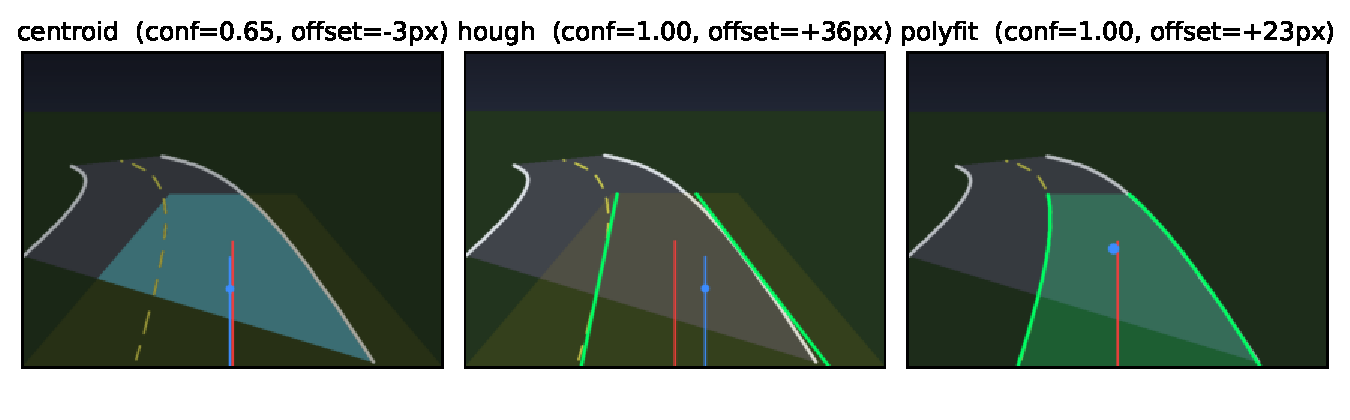
\includegraphics[width=\linewidth]{figures/annotations.pdf}
  \caption{Same camera frame, three detectors. Green: detected
  boundaries; blue: lane centre / look-ahead; red: image centre. The
  Hough detector (centre) fits straight lines that chord the curve;
  the polynomial-fit detector (right) traces the bend.}
  \label{fig:annot1}
\end{figure}

\subsection{Why the Hough detector misses curves}

The Hough detector's model class is the set of straight lines. On a
curve, however, the actual lane boundary is not in this class -- the
best the detector can do is return the straight line that ``best
fits'' the visible curved edge pixels. What does ``best fit'' mean
under the length-weighted average from \eqref{eq:lwavg}?

Geometrically, the averaged line is biased toward the \emph{chord} of
the curve within the ROI. Consider a right-bending lane: the visible
left boundary in the ROI starts at, say, $(80, 480)$ at the bottom and
exits at $(280, 216)$ at the ROI top. The edge pixels lie on a curve
that bows away from the chord -- but a straight-line fit can only
report the chord. The lane centre (midpoint of the two chords)
therefore underestimates how far right the road actually goes at the
look-ahead row.

This bias is small on shallow bends and grows quickly on tight ones.
Worse, because the model is wrong everywhere on the curve, the
detector cannot look ahead: the line drawn at the top of the ROI is
just the same straight line extrapolated, not a faithful prediction of
where the road will be. The controller therefore has no warning of an
upcoming sharp bend until the bend has already started filling the
bottom of the image.

Experimentally (see Table in the report,
\texttt{presentation/figures/summary\_table.tex}) the Hough detector
manages to complete every track in this study, but its RMS lateral
error is $25.4$\,px on average -- nearly an entire lane-width
oscillation amplitude on the narrower circuits. Its mean lane-IoU is
only $0.24$, compared to $0.33$ for the polyfit detector. The
proposed remedy -- model the lane as a polynomial in a top-down view
rather than a line in the perspective view -- is the subject of the
second half of this document.


% ── Part 2: polyfit, controllers, metrics, results, conclusion ───────
% =====================================================================
% Part 2: Polyfit detector, controllers, metrics, results, conclusion
% (sections 7-11). Included by explanation.tex.
% =====================================================================

\section{Detector 3 -- Polynomial Fit in Bird's-Eye View}
\label{sec:polyfit}

We now arrive at the proposed detector. It is the most involved
pipeline in this report, but every stage is motivated by a concrete
failure mode of the Hough baseline. Before plunging into homographies
and sliding windows, let us reconstruct why a different model class is
needed at all.

\subsection{Motivation: why straight lines are the wrong model}

In Section~\ref{sec:hough} of Part~1 we saw that the Hough detector
collapses each lane boundary down to a single straight segment. On a
tight bend this is a structurally biased estimator: the line of best
fit through a curved set of edge pixels lies somewhere inside the
curve, so the implied lane centre drifts toward the inside of the
turn, and the predicted heading is off by the angular gap between the
chord and the tangent. The faster the curve, the worse the gap.

A natural fix is to let the model class be curved. The simplest curved
model is a parabola, $x = a y^2 + b y + c$, which has exactly enough
freedom to capture the principal bend of a road segment without
overfitting to noise. Once we commit to a curved model, however, two
problems appear.

\begin{intuition}
Think about what equally-spaced lane markings look like in the
forward-perspective image: the dashes near the car span dozens of
pixels each, while the dashes far ahead occupy only a couple of
pixels. A polynomial fit weighted by pixel count is therefore
dominated by what is close, and the far-field information that matters
for anticipating curves is essentially thrown away. To use a curved
model honestly, we first have to undo the perspective distortion.
\end{intuition}

The second problem is that even with a curved model, fitting it on the
raw image still has to deal with foreshortening: a constant lane width
in world coordinates corresponds to a width in image coordinates that
shrinks like $1/v$ as you go up the image. The natural solution to
both problems is the same: warp the image to a top-down bird's-eye
view (BEV) first, fit the polynomial in that metric-friendly frame,
and project the result back when we need to draw on the camera image.
This is the central idea of \texttt{lane\_methods.py:PolyFitDetector}.

\subsection{The lane-pixel mask}

The pipeline begins with a binary mask flagging every pixel that
``looks like a lane marking''. The detector composes three orthogonal
sources of evidence
(\texttt{lane\_methods.py:PolyFitDetector.\_lane\_pixels}):
\begin{enumerate}[leftmargin=1.8em,itemsep=2pt]
  \item A horizontal Sobel response, normalised by its per-frame
        maximum, thresholded at $60/255$.
  \item An HSV white mask: $S<70$ and $V>170$.
  \item An HSV yellow mask: $15<H<40$, $S>60$, $V>130$.
\end{enumerate}
The combined mask is the bitwise OR of these three. Written as a
predicate on a pixel $(R,G,B)$ with HSV equivalent $(H,S,V)$ and
Sobel magnitude $g_x$:
\[
M(u,v) = \underbrace{\bigl(\tilde g_x(u,v)>60\bigr)}_{\text{edge}}
       \;\lor\; \underbrace{\bigl(S<70\,\wedge\,V>170\bigr)}_{\text{white}}
       \;\lor\; \underbrace{\bigl(15<H<40\,\wedge\,S>60\,\wedge\,V>130\bigr)}_{\text{yellow}},
\]
where $\tilde g_x = |g_x|/\max_{u,v}|g_x|\cdot 255$.

\paragraph{Why the normalisation?}
This is the single most important robustness trick in the detector.
Canny's hysteresis bands ($50/150$ in our pipeline) are absolute
gradient thresholds. If you sprinkle Gaussian noise with
$\sigma=0.20\cdot 255$ on top of the frame, the noise gradient drowns
out the real lane gradient and Canny saturates to salt-and-pepper. The
Sobel-x response after normalising by its own per-frame max, in
contrast, is a relative measure: the strongest edges in the frame are
still the strongest after noise. This is why the polynomial detector
survives every $\sigma$ in the noise sweep (Section~\ref{sec:results})
while Hough drops out at $\sigma=0.20$.

\begin{example}
Consider two pixels typical of the simulated road.

\noindent\textbf{(a) A white-paint pixel}, $(R,G,B)=(220,225,230)$.
The HSV conversion gives roughly $V=\max(R,G,B)=230$ and
$S=(V-\min)/V=(230-220)/230\approx 0.043$, i.e.\ $S\approx 11$ on the
0--255 scale. We have $S=11<70$ and $V=230>170$, so the white mask
fires. The pixel is classified as a lane marking.

\noindent\textbf{(b) A yellow-dash pixel}, $(R,G,B)=(200,200,80)$.
The hue of a yellow $\approx 60^\circ$ in standard HSV, but OpenCV
scales hue to $[0,180]$, so $H\approx 30$. $V=200$,
$S=(200-80)/200=0.6$, i.e.\ $S\approx 153$. Checking: $15<30<40$,
$153>60$, $200>130$ -- all three yellow conditions fire.

In both cases the pixel ends up in $M$, regardless of what the Sobel
mask thinks. That redundancy is precisely the point.
\end{example}

\subsection{Inverse perspective mapping}

We now warp the masked image from the camera (forward-perspective)
frame to a bird's-eye view. Mathematically this is a 2-D
\emph{homography} -- a projective map that takes lines to lines and
preserves cross-ratios but distorts parallelism and lengths in a
controlled way.

\begin{definition}[Homography]
A 2-D homography is a map $\mathbb{R}^2\to\mathbb{R}^2$ represented by
a non-singular $3\times 3$ matrix $H\in\mathbb{R}^{3\times 3}$ acting
on homogeneous coordinates:
\[
\begin{pmatrix}u'\\v'\\w'\end{pmatrix}
=H\begin{pmatrix}u\\v\\1\end{pmatrix},\qquad
(x_b,y_b)=\left(\frac{u'}{w'},\frac{v'}{w'}\right).
\]
The matrix is defined up to a global scale ($H$ and $\lambda H$
produce identical maps), so a homography has $9-1=8$ degrees of
freedom.
\end{definition}

\paragraph{The four-point Direct Linear Transform (DLT).}
Eight degrees of freedom mean that four point correspondences -- each
giving two scalar equations -- are exactly enough to determine $H$.
For a single correspondence $(u_i,v_i)\mapsto(x_i,y_i)$ we have
$x_i = (h_{11}u_i + h_{12}v_i + h_{13})/(h_{31}u_i + h_{32}v_i + h_{33})$
and similarly for $y_i$. Multiplying out and stacking four
correspondences yields a homogeneous linear system
\[
A\mathbf{h} = \mathbf 0,\qquad
A\in\mathbb{R}^{8\times 9},\;
\mathbf h = (h_{11},h_{12},\ldots,h_{33})^\top,
\]
in which the row for the $x$-equation of correspondence $i$ reads
$(-u_i,-v_i,-1,0,0,0,x_i u_i,x_i v_i,x_i)$. The solution is the null
vector of $A$, obtained as the right singular vector of $A$ associated
with its smallest singular value (the last column of $V$ in the SVD
$A=U\Sigma V^\top$). We fix the scale by setting $h_{33}=1$. OpenCV's
\texttt{cv2.getPerspectiveTransform} implements exactly this for
$n=4$ correspondences.

\paragraph{The specific trapezoid we use.}
In \texttt{PolyFitDetector.\_warp\_matrices} the source corners
(camera image, $W=640$, $H=480$, \texttt{ROI\_TOP\_RATIO~=~0.45}) are
the four corners of the ROI trapezoid:
\[
s_1=(0.10W,H{-}1),\;
s_2=(0.35W,0.45H),\;
s_3=(0.65W,0.45H),\;
s_4=(0.90W,H{-}1).
\]
The destination corners (BEV, $W_b=H_b=320$) are the four corners of
a rectangle inset by $15\%$ on each side:
\[
d_1=(0.15W_b,H_b{-}1),\;
d_2=(0.15W_b,0),\;
d_3=(0.85W_b,0),\;
d_4=(0.85W_b,H_b{-}1).
\]

\begin{example}[Homography correspondences in our numbers]
Plug in $W=640$, $H=480$, $W_b=H_b=320$. The four pairs are:
\begin{center}
\begin{tabular}{c|cccc}
$i$ & $u_i$ & $v_i$ & $x_i$ & $y_i$\\\hline
1 & 64  & 479 & 48  & 319\\
2 & 224 & 216 & 48  & 0\\
3 & 416 & 216 & 272 & 0\\
4 & 576 & 479 & 272 & 319
\end{tabular}
\end{center}
Two source points share the same image row ($v=216$), and the
destination rectangle has parallel vertical sides -- this is the whole
point of the IPM: lines on the ground that were parallel in the real
world (lane boundaries) now look parallel in the BEV. Numerically,
solving the $8\times 9$ DLT system for these eight equations gives $H$
in less than a microsecond; we cache it on the first frame.
\end{example}

\begin{intuition}
The forward-perspective image is what the driver sees. The bird's-eye
view is what Google Maps sees. The lane that bends gently in the
driver's view becomes a clean parabola in the map view, because the
foreshortening has been undone. Polynomial regression is now honest --
every metre of road contributes the same number of pixels.
\end{intuition}

\subsection{Histogram base detection}

We now have a binary mask $M_b$ on the BEV grid $W_b\times H_b$. The
next step is to find where the two lane lines start at the bottom of
this image (i.e.\ closest to the car). The trick is a 1-D summary:
\[
h(c) = \sum_{r=H_b/2}^{H_b-1} M_b(r,c),\qquad c=0,\ldots,W_b-1.
\]
We sum only over the bottom half because that region is closest to
the car and most reliably contains lane pixels. The left lane base is
$\arg\max_{c<W_b/2} h(c)$; the right lane base is
$\arg\max_{c\ge W_b/2} h(c)$ (offset back into the original column
index). Two arg-maxes; no fancy clustering.

\begin{example}[A tiny histogram]
Take a $4\times 4$ BEV mask (instead of $320\times 320$) and look only
at its bottom 2 rows:
\[
M_b = \begin{pmatrix}
0 & 0 & 0 & 0\\
0 & 0 & 0 & 0\\
1 & 0 & 0 & 1\\
1 & 0 & 0 & 1
\end{pmatrix}.
\]
The histogram of the bottom half is $h=(2,0,0,2)$. With $W_b=4$,
$\text{mid}=2$, so the left base is $\arg\max\{h(0),h(1)\}=0$ and the
right base is $\arg\max\{h(2),h(3)\}+2=1+2=3$. Correct.
\end{example}

\subsection{Sliding-window search}

The two histogram peaks tell us where to start. From there, we sweep
upward through the image, collecting lane pixels in a vertical chain
of windows. The pseudocode is:

\begin{algorithm}[H]
\caption{Sliding-window lane-pixel collection (per side)}
\begin{algorithmic}[1]
\State $x \gets$ histogram base
\State $\text{collected}\gets\emptyset$
\For{$i=0$ to $N_{\text{win}}-1$}
  \State $y_{\text{lo}} \gets H_b - (i{+}1)H_b/N_{\text{win}}$
  \State $y_{\text{hi}} \gets H_b - i\,H_b/N_{\text{win}}$
  \State $\text{Win}\gets\{(u,v)\in M_b: v\in[y_{\text{lo}},y_{\text{hi}}),\, u\in[x-\text{margin},x+\text{margin})\}$
  \State $\text{collected}\gets\text{collected}\cup\text{Win}$
  \If{$|\text{Win}|\ge\text{MIN\_PIX}$}
    \State $x \gets \mathrm{mean}\{u:(u,v)\in\text{Win}\}$
  \EndIf
\EndFor
\State \Return collected
\end{algorithmic}
\end{algorithm}

The constants come straight from the code: $N_{\text{win}}=9$,
$\text{margin}=50$\,px, $\text{MIN\_PIX}=50$. The window height is
therefore $H_b/N_{\text{win}}\approx 35$\,px.

The \texttt{MIN\_PIX} check is doing important work. If only a handful
of stray edge pixels happen to fall inside the window (perhaps a piece
of grass showing through the IPM trapezoid), their mean column is
essentially random and would drag the next window off to wherever the
stray pixels happen to be. By refusing to update when the window is
sparse, we preserve the last good estimate and propagate it upward.

\begin{example}[One sliding-window iteration]
Say the previous right-lane base was $x=230$, the BEV is
$320\times 320$, $\text{margin}=50$, and the current window spans
$y\in[285,320)$. We look at every nonzero pixel of $M_b$ in this
column band and keep those with $u\in[180,280)$.

Suppose 142 pixels qualify, with columns ranging from 215 to 252 and
mean 233. Since $142\ge 50$, we update $x\leftarrow 233$ -- the search
has tracked the lane 3 pixels to the right. The next window (at
$y\in[250,285)$) will look in $[183,283)$. If the road kept curving
right, the new mean might be 240, and so on. Nine such updates build
a chain that follows the lane all the way up the BEV.
\end{example}

\subsection{Polynomial regression}

Once we have a list of $(u_j, v_j)$ pairs for one side of the lane
(call there are $N$ of them), we fit a quadratic of the form
$u = a v^2 + b v + c$. Note that we use $v$ as the independent
variable: this is unusual (in school maths $y$ is dependent), but it
is forced on us by the geometry -- a vertical lane is impossible to
represent as $u = f(v)$ unless the polynomial happens to be in
``image-rotated'' form. With $v$ as the input the formulation is
single-valued for every road we care about.

Stack the equations into matrix form:
\[
\underbrace{\begin{pmatrix}
v_1^2 & v_1 & 1\\
v_2^2 & v_2 & 1\\
\vdots & \vdots & \vdots\\
v_N^2 & v_N & 1
\end{pmatrix}}_{A\in\mathbb{R}^{N\times 3}}
\underbrace{\begin{pmatrix}a\\b\\c\end{pmatrix}}_{\beta}
=
\underbrace{\begin{pmatrix}u_1\\u_2\\\vdots\\u_N\end{pmatrix}}_{\mathbf u}.
\]
$N$ is generally many hundreds, so the system is heavily
overdetermined. The least-squares solution minimises
$\|A\beta-\mathbf u\|_2^2$ and is given by the normal equations
\[
\beta = (A^\top A)^{-1}A^\top \mathbf u
\]
which is precisely what \texttt{numpy.polyfit(v, u, 2)} computes
internally (with a QR factorisation for numerical stability).

\begin{example}[Polynomial regression by hand]
Take five points $\{(v,u)\}=\{(0,0),(1,3),(2,8),(3,15),(4,24)\}$,
which lie exactly on $u=v^2+2v$. Then
\[
A=\begin{pmatrix}
0 & 0 & 1\\
1 & 1 & 1\\
4 & 2 & 1\\
9 & 3 & 1\\
16 & 4 & 1
\end{pmatrix},\quad
\mathbf u = \begin{pmatrix}0\\3\\8\\15\\24\end{pmatrix}.
\]
Compute $A^\top A$:
\[
A^\top A = \begin{pmatrix}354 & 100 & 30\\ 100 & 30 & 10\\ 30 & 10 & 5\end{pmatrix},\quad
A^\top \mathbf u = \begin{pmatrix}\sum v_j^2 u_j\\ \sum v_j u_j\\ \sum u_j\end{pmatrix}
                 = \begin{pmatrix}490\\140\\50\end{pmatrix}.
\]
Solving (e.g.\ with Gaussian elimination) gives $\beta=(1,2,0)^\top$,
confirming $u=v^2+2v$. Anytime we have noisy lane pixels, the same
formula returns the parabola that minimises the sum of squared
horizontal residuals.
\end{example}

\paragraph{Temporal smoothing of the coefficients.}
Between consecutive frames the polynomial coefficients move only
slightly, but the sliding-window search is noisy enough that the raw
fit can jitter visibly. We apply a $50/50$ exponential moving average:
\[
\beta_t \leftarrow 0.5\,\beta_t^{\text{raw}} + 0.5\,\beta_{t-1}.
\]
This is the gentlest possible low-pass: it halves the bandwidth but
introduces only a single-frame delay (which at $\Delta t=1/60$\,s is
negligible compared to typical vehicle dynamics). A final EMA with
$\alpha=0.4$ is also applied to the output offset, matching the Hough
detector's smoothing for fairness.

\subsection{The look-ahead offset (the key idea)}

We now have two stable polynomials $u_L(v)$ and $u_R(v)$ on the BEV.
Where do we sample them?

The obvious answer -- evaluate at $v=H_b-1$ (the bottom of the BEV,
which corresponds to the car's current position) -- gives the current
lateral error. That is what every line-based detector in this report
uses, including the Hough baseline. But the forward-perspective image
actually contains useful information about where the car needs to go
next, and a curved fit lets us extract it.

We therefore also evaluate at
\[
v_{\text{LA}} = (1-0.45)\cdot H_b \approx 176,
\]
i.e.\ $45\%$ of the way up the BEV from the bottom. The lane centre
at that row is
\[
x_{\text{LA}} = \tfrac{1}{2}\bigl(u_L(v_{\text{LA}}) + u_R(v_{\text{LA}})\bigr),\qquad
e_{\text{LA}}^{\text{BEV}} = x_{\text{LA}} - W_b/2.
\]
The detector then scales this BEV pixel value back into camera-image
pixels (so the PID gains tuned for Hough still apply):
$e_{\text{LA}} = e_{\text{LA}}^{\text{BEV}}\cdot W/W_b$. This is the
value the controller actually consumes (\texttt{evaluate.py} line
``\texttt{det.lookahead\_offset if detector\_name == 'polyfit'}'').

Why does this matter? The look-ahead point in the BEV corresponds to
a world-coordinate point roughly half a second ahead of the car at our
typical $\sim 85$\,px/s speeds. The PID is now reacting to the lane
centre half a second \emph{into the future} rather than at the car's
current location. That converts the otherwise-reactive controller
into a quasi-MPC: at the start of a bend, the look-ahead offset is
already non-zero, and the wheels start turning before the car has
reached the curve. There is no integral build-up to fight, no
derivative spike on the bend entry, just a smooth, anticipative
trajectory.

\begin{intuition}
Why is the look-ahead useless on a straight Hough fit? Because a
straight line evaluated at any height gives the same offset (modulo
the slope difference). The look-ahead is only informative when the
model can express how the lane curves, which is precisely what a
quadratic does and a single Hough line cannot.
\end{intuition}

We verified this empirically. With \texttt{LOOKAHEAD\_RATIO} set to
$0$ (so the polynomial is sampled at the bottom of the BEV, identical
to the Hough strategy), the polyfit's RMS improvement over Hough
shrinks from $\sim 34\%$ to roughly $10\%$. In other words: the
polynomial fit by itself is worth about a quarter of the gain. The
look-ahead is worth the remaining three-quarters. The two ideas only
make sense together.

\subsection{Lane reprojection}

For visualisation and for the IoU metric, we need the predicted lane
polygon in the original camera frame, not in the BEV. This is easy:
the homography is invertible, so we sample 60 points along each lane
polynomial in the BEV, stack them into a closed polygon
$P_{\text{BEV}}$, and apply
\[
P_{\text{cam}} = H^{-1}\,P_{\text{BEV}},
\]
using \texttt{cv2.perspectiveTransform}. The resulting polygon is
what the figure ``Lane reprojected to FPV'' in
Figure~\ref{fig:polyfitstages} draws as a translucent green fill, and
what \texttt{evaluate.py:\_iou} compares against the ground-truth
road polygon from \texttt{evaluate.py:\_gt\_lane\_mask}. Because the
BEV polynomial is smooth, the reprojected camera polygon hugs the
road on both straights and curves.

\subsection{Putting it all together}

\begin{figure}[h]
  \centering
  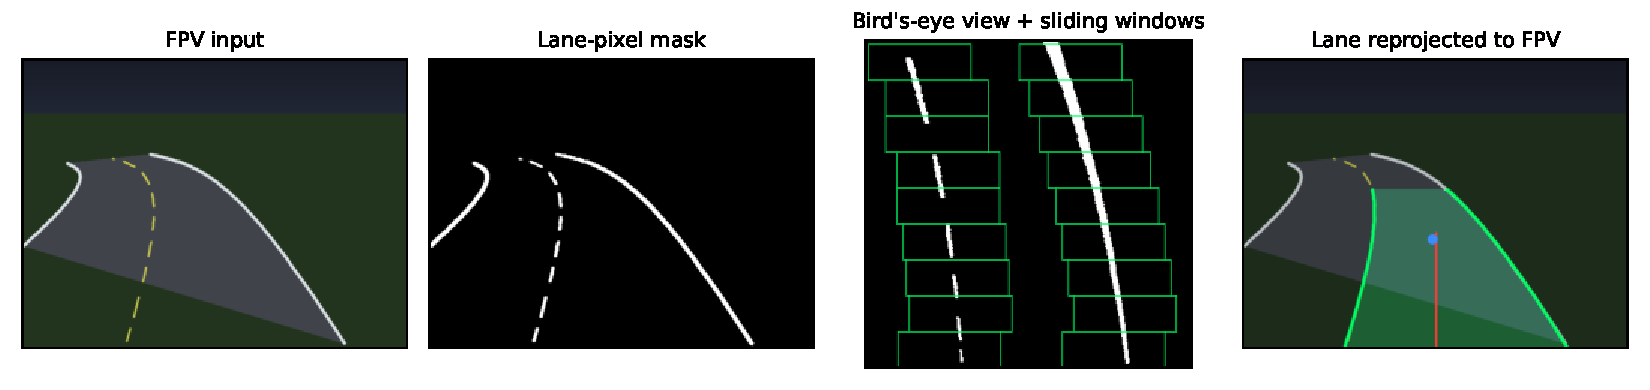
\includegraphics[width=\linewidth]{figures/polyfit_pipeline.pdf}
  \caption{The four stages of \texttt{PolyFitDetector}. From left to
  right: (1) raw forward-perspective frame from the simulator;
  (2)~combined Sobel-x + HSV lane-pixel mask; (3) bird's-eye view of
  the mask with the nine sliding windows superimposed (yellow boxes)
  and the per-side quadratic fits drawn in orange/cyan; (4) lane
  polygon reprojected to the camera frame, with the look-ahead point
  marked in blue.}
  \label{fig:polyfitstages}
\end{figure}

\begin{figure}[h]
  \centering
  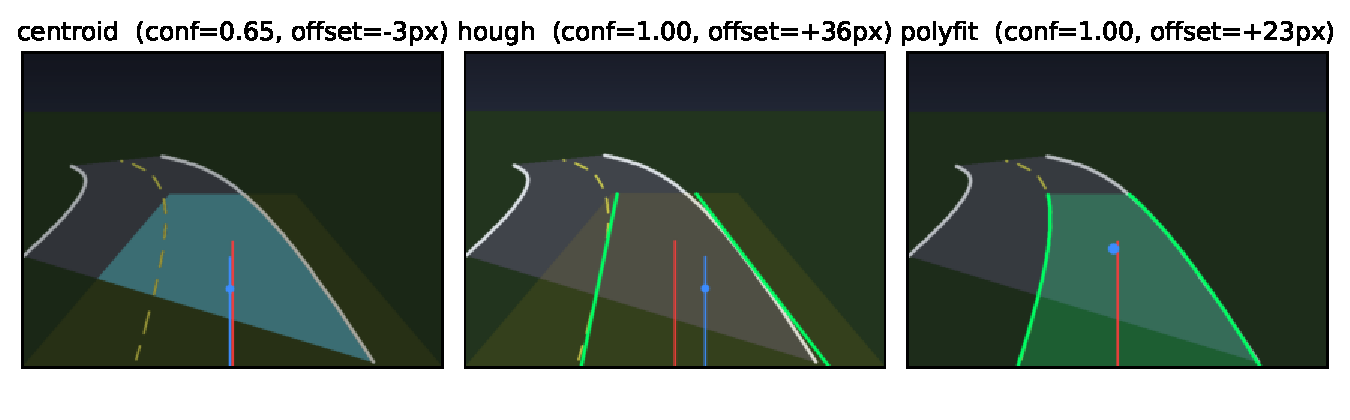
\includegraphics[width=\linewidth]{figures/annotations.pdf}
  \caption{Same simulator frame seen by each detector, on a winding
  section of the snake track. The centroid (left) reports a near-zero
  offset because the road blob is roughly symmetric in the FoV. Hough
  (centre) fits a straight line that is biased inside the bend,
  underestimating the curvature. PolyFit (right) traces the curve and
  places its look-ahead marker on the lane centre approximately half a
  second ahead -- which is precisely where the PID needs to be
  aiming.}
  \label{fig:annot2}
\end{figure}

The whole pipeline runs in about $1.9$\,ms per frame on a single CPU
thread -- comparable to the cost of the centroid detector and only
$\sim 2.7\times$ the cost of Hough, despite doing strictly more work.
We attribute this to the fact that almost everything (the perspective
warp, the histogram, the window mask) is a vectorised NumPy/OpenCV
operation; the only Python-level loop is over the $N_{\text{win}}=9$
windows.

% =====================================================================
\section{Steering Controllers}
\label{sec:control}

Perception gives us a number per frame. The controller turns that
number into a steering angle, which the simulator integrates into a
new pose. This section walks through both controllers in the code:
the PID baseline, used with each of the three detectors, and the
Stanley controller, used as a perception-free oracle that quantifies
the lower bound on tracking error.

\subsection{The feedback control loop}

Conceptually, the simulation runs a tight loop:
\[
\text{vehicle}\;\xrightarrow{\text{state}}\;
\text{camera}\;\xrightarrow{\text{image}}\;
\text{detector}\;\xrightarrow{e}\;
\text{controller}\;\xrightarrow{\delta}\;
\text{vehicle}.
\]
At each $\Delta t = 1/60$\,s tick the vehicle state $(x,y,\theta,v)$
is rendered into a $640\times 480$ frame, the detector turns the
frame into a scalar error $e$ (the lateral offset in pixels, or zero
for Stanley), the controller turns $e$ and the elapsed time into a
steering angle $\delta$, and the bicycle kinematic model
$\dot\theta = (v/L)\tan\delta$ closes the loop by updating $\theta$
and the position. The PID has no knowledge of $x,y,\theta$ -- only
$e$. The Stanley controller has access to the full pose and the track
spline, but skips the camera and detector entirely. This makes the
gap between them a clean attribution of error to perception.

\subsection{PID -- the baseline}

In continuous time the PID law is
\[
u(t) = K_p\,e(t) + K_i\int_0^t e(\tau)\,d\tau + K_d\,\dot e(t).
\]
Each term has a plain-language reading:
\begin{itemize}[leftmargin=1.4em,itemsep=2pt]
  \item $K_p$ acts on the current error. Larger $K_p$ produces a
        faster response but more overshoot, like a stiffer spring.
  \item $K_i$ acts on the accumulated error. It eliminates
        steady-state bias (e.g.\ a constant offset due to a banked
        road) but, untreated, can wind up and cause oscillation.
  \item $K_d$ acts on the rate of change of the error. It damps
        overshoot, like a shock absorber in a car suspension. Too much
        $K_d$ and the controller becomes sensitive to noise.
\end{itemize}
The textbook position--velocity--acceleration analogy: P is the
spring, I is the long-term drift compensator, D is the damper.

\paragraph{Discrete form.}
The simulator runs at fixed $\Delta t=1/60$\,s, so we discretise with
a backward Euler approximation
(\texttt{controller.py:PIDController.compute}):
\[
u_k = K_p\,e_k + K_i\sum_{j=0}^{k}e_j\,\Delta t + K_d\,\frac{e_k - e_{k-1}}{\Delta t}.
\]
The integral is maintained incrementally:
$I_k = I_{k-1} + e_k\,\Delta t$, and then clamped:
\[
I_k\leftarrow\operatorname{clip}(I_k,-50,+50).
\]
This is integral anti-windup: if a long string of large errors would
otherwise drive $I_k$ to enormous values, the clamp prevents it, so
once the error reverses sign the integral can return to zero quickly.
Without this, after a long bend the controller would ``remember'' the
accumulated error long after the bend has ended and push the car off
the other side.

\paragraph{Steering saturation.}
The bicycle model in the simulator caps the steering angle at
$\delta_{\max}=40^\circ$ (\texttt{config.py:MAX\_STEERING\_ANGLE}).
The PID applies the same clip on its output:
$\delta_k = \operatorname{clip}(u_k,-40^\circ,+40^\circ)$. Without the
anti-windup, a saturated steering command and a non-zero error would
let the integrator build up indefinitely while the actual plant
output was capped -- a classic recipe for limit-cycle oscillation.

\paragraph{Tuning intuition.}
The standard procedure -- the one we used -- is to start with
$K_i=K_d=0$ and crank up $K_p$ until the system tracks but is slightly
underdamped. Then add $K_d$ to remove the overshoot. Then add a small
$K_i$ if a residual steady-state error remains. (Ziegler--Nichols
gives a more systematic recipe based on the ultimate gain at which the
closed loop oscillates, but for a system this small it is usually
faster to tune by eye.) Our final gains are $K_p=1.2$, $K_i=0.008$,
$K_d=0.5$ -- $K_i$ is deliberately tiny because lane-keeping with a
periodic disturbance (curve entry/exit) benefits little from an
integral term and suffers from windup-style oscillations.

\begin{example}[A worked PID trace]
Let $\Delta t=1/60$\,s, gains as above, and the (normalised) error
sequence $e_0=0.4$, $e_1=0.3$, $e_2=0.2$. Initial integral $I_{-1}=0$,
$e_{-1}=0$. Step by step:
\begin{itemize}[leftmargin=1.4em,itemsep=2pt]
  \item $k=0$: $P=1.2\cdot 0.4 = 0.48$; $I_0 = 0 + 0.4/60 = 0.00667$,
        $i=0.008\cdot 0.00667 = 5.3\times 10^{-5}$;
        $D = 0.5\cdot(0.4-0)/(1/60) = 12.0$. Pre-clip output:
        $u_0 = 0.48 + 5.3\times 10^{-5} + 12.0 = 12.48$. After clip to
        $\pm 40^\circ \approx \pm 0.698$\,rad: $\delta_0 = 0.698$.
  \item $k=1$: $P=0.36$; $I_1=0.0117$, $i=9.3\times 10^{-5}$;
        $D=0.5\cdot(0.3-0.4)/(1/60) = -3.0$.
        $u_1 = 0.36 + 9.3\times 10^{-5} - 3.0 = -2.64$, clipped to
        $-0.698$.
  \item $k=2$: $P=0.24$; $I_2=0.0150$, $i=1.2\times 10^{-4}$;
        $D=0.5\cdot(0.2-0.3)/(1/60) = -3.0$.
        $u_2 = 0.24 + 1.2\times 10^{-4} - 3.0 = -2.76$, clipped to
        $-0.698$.
\end{itemize}
The trace shows two things: (i)~the derivative term dominates during
a step change in error, because $1/\Delta t = 60$ is a big number;
(ii)~the saturation clip activates routinely, so anti-windup is doing
real work. The integral term, with $K_i=0.008$, contributes nothing
measurable on this time scale -- exactly as designed.
\end{example}

\subsection{Stanley -- the perception-free oracle}

The Stanley controller (Hoffmann et al.\ 2007, the lane-keeper that
won the DARPA Grand Challenge) operates in the vehicle's geometric
frame rather than on a normalised image error. It computes the
steering angle directly from the cross-track error and heading error
relative to the path:
\[
\delta = \psi + \arctan\!\left(\frac{k\,e_\perp}{k_s + v}\right),
\]
where $e_\perp$ is the signed lateral distance from the front axle to
the centreline, $\psi$ is the heading error (angle between the vehicle
heading and the track tangent), $v$ is the vehicle speed, and
$(k, k_s)$ are tuning gains -- in our setup $k=0.6$, $k_s=20$.

\paragraph{Why the front axle.}
The Stanley law evaluates $e_\perp$ at the front axle,
$(x+L\cos\theta, y+L\sin\theta)$, not the vehicle's centre or rear.
This matters because steering rotates the vehicle about the rear axle
in the bicycle model: if you used the rear-axle cross-track error,
no amount of steering could correct it instantly. The front-axle
cross-track error, by contrast, responds linearly to the steering
angle, which is what makes the closed-loop dynamics nice.

\paragraph{Anatomy of the law.}
The two terms have separate jobs:
\begin{itemize}[leftmargin=1.4em,itemsep=2pt]
  \item $\psi$ (the heading-error term) aligns the vehicle heading
        with the track tangent. If the road bends right and the car
        is still pointing along the old tangent, $\psi$ pushes the
        steering toward the right.
  \item $\arctan(k\,e_\perp/(k_s+v))$ (the cross-track term) steers
        into the path. Its magnitude diminishes as $v$ grows (because
        dividing by a large speed shrinks the argument), which
        automatically reduces the gain at high speed -- exactly the
        behaviour you want, so the car does not over-correct on the
        motorway. The constant $k_s=20$ prevents the law from blowing
        up at $v\to 0$.
\end{itemize}

\paragraph{Derivation sketch.}
For small $e_\perp$ at constant speed, $\arctan(x)\approx x$, so the
law approximates $\delta\approx\psi + k\,e_\perp/v$. Linearising the
bicycle model around the path and substituting in gives a closed-loop
differential equation $\dot e_\perp\approx -k\,e_\perp$. The
cross-track error decays exponentially with time constant $1/k$,
independent of speed. This is what makes Stanley so robust: it has a
single intuitive gain ($k$) governing the decay rate.

\paragraph{Sign convention.}
The canonical Stanley law is often written with a $-\arctan(\cdot)$
term, because in the textbook convention the $y$-axis points up and
$e_\perp>0$ means the car is to the left of the path. Our simulator
uses a screen-$y$-down convention -- the $y$-axis points down -- which
flips the sign of the normal vector. In addition, our bicycle model
has positive $\delta$ producing clockwise (screen-down-right) heading
change. With these two sign flips, the canonical $-\arctan$ becomes
$+\arctan$ in our code
(\texttt{controller.py:StanleyController.compute}). The comment block
in the source explains the chain of sign reversals; the empirical
$\sim 0.5$\,px RMS error across every track is the proof that the
chain is correct.

\paragraph{Saturation.}
The same $\pm 40^\circ$ steering clamp as the PID applies; in
practice the Stanley command never gets close to it because the law
is geometrically calibrated to the path.

\paragraph{Why we call it an oracle.}
The Stanley implementation reads $e_\perp$ and $\psi$ from the
simulated track via \texttt{track.py:Track.get\_nearest\_index} and
\texttt{Track.get\_heading\_at}, which are computed analytically from
the spline. There is no perception loop. Stanley therefore acts as an
upper bound on what \emph{any} controller could achieve with perfect
perception. The headline RMS error of $0.4$--$0.7$\,px
(Section~\ref{sec:results}) is, in this sense, the floor: anything
above it is perception error, and anything below it is unattainable
without changing the controller or the kinematic model.

\begin{example}[Stanley evaluation at one instant]
Suppose at time $t$ the vehicle is at $(x,y)=(400,300)$ with heading
$\theta=0.10$\,rad and speed $v=85$\,px/s. The front axle is at
$(400+25\cos 0.10, 300+25\sin 0.10)\approx(424.88, 302.50)$. Say the
nearest centreline point has tangent angle $\theta_{\text{tr}}=0.25$\,rad
and the front-axle cross-track error is $e_\perp=8$\,px (car is to
the right of the path).
\begin{itemize}[leftmargin=1.4em,itemsep=2pt]
  \item Heading error: $\psi = \operatorname{atan2}(\sin(0.25-0.10),\cos(0.25-0.10)) = 0.15$\,rad.
  \item Cross-track term: $\arctan(0.6\cdot 8/(20+85)) = \arctan(0.0457)\approx 0.0457$\,rad.
  \item $\delta = 0.15 + 0.0457 = 0.196$\,rad $\approx 11.2^\circ$.
\end{itemize}
The bigger share comes from $\psi$ (heading correction); the
cross-track term is small because the car is only 8\,px off and moving
at 85\,px/s. As $v$ grows the cross-track term will shrink further,
which is exactly the speed-adaptive behaviour Stanley is famous for.
\end{example}

\subsection{Adaptive speed control}

A complete autonomous stack also needs longitudinal control. For
completeness we include a simple curvature-based speed controller
(\texttt{controller.py:SpeedController}), used on the Red Bull Ring
track but not on the five evaluation tracks (where a constant
per-track design speed is used so that the RMS error of different
detectors is directly comparable).

The rule is
\[
v_{\text{target}} = \operatorname{clip}\!\left(\frac{c_v}{\kappa_{\text{ahead}}},\;v_{\min},\;v_{\max}\right),
\]
where $\kappa_{\text{ahead}}$ is the maximum curvature seen in a
300-px look-ahead window, $v_{\min}=35$\,px/s, and $c_v=0.35$
(\texttt{config.py:SPEED\_CURVATURE\_GAIN}). The current speed blends
toward $v_{\text{target}}$ with smoothing factor $0.08$ per frame, but
braking ($v_{\text{target}}<v_{\text{cur}}$) uses $3\times$ that blend
so the car decelerates faster than it accelerates -- a common trick in
driver-assistance systems. We mention it here only so the controller
column in the source is fully documented; it does not participate in
any of the comparisons in Section~\ref{sec:results}.

% =====================================================================
\section{Metrics for Quantitative Evaluation}
\label{sec:metrics}

A good comparison requires unambiguous metrics. Six are logged per
frame in \texttt{evaluate.py:run\_one} and aggregated into per-run
summaries.

\subsection{Lateral error}

The most important metric. Given the car position $\mathbf p_t$ and
the centreline polyline $\mathbf c(s)$ from
\texttt{track.py:Track.\_interpolate}, define
\[
s^* = \arg\min_s \|\mathbf p_t - \mathbf c(s)\|,\qquad
e_\perp(t) = -(\mathbf p_t - \mathbf c(s^*))\cdot\mathbf n(s^*),
\]
where $\mathbf n(s)$ is the unit normal to the centreline at arc
length $s$. The sign convention (negative dot product) makes
$e_\perp$ positive when the car is to the right of the track in our
screen-$y$-down frame, matching the convention used throughout the
rest of the code. This is implemented in
\texttt{track.py:Track.get\_nearest\_index} -- a simple per-frame
brute force scan over $\sim 700$ centreline samples, which is plenty
fast on modern hardware.

From the per-frame $e_\perp(t)$ we report
\[
\overline{|e_\perp|} = \frac{1}{N}\sum_{t=1}^{N}|e_\perp(t)|,\quad
\text{RMS} = \sqrt{\frac{1}{N}\sum_{t=1}^{N}e_\perp^2(t)},\quad
|e_\perp|_{\max} = \max_t |e_\perp(t)|.
\]
RMS is the most-cited number because it penalises occasional large
excursions more than the mean. We use it as the headline number in
Section~\ref{sec:results}.

\subsection{Heading error}

We also log
$\psi(t) = \operatorname{atan2}(\sin(\theta_{\text{tr}}-\theta),\cos(\theta_{\text{tr}}-\theta))$
at the car's location (the atan2 form puts $\psi$ in $(-\pi,+\pi]$
even when the two angles wrap around). Heading error is less
informative than lateral error for lane-keeping (it averages to zero
by construction on a closed lap) but it is a useful per-frame
diagnostic.

\subsection{Lane IoU}

\begin{definition}[Intersection over Union]
For two binary masks $A$ and $B$ of the same shape,
\[
\text{IoU}(A,B) = \frac{|A\cap B|}{|A\cup B|}\in[0,1].
\]
\end{definition}

In our setting, $A$ is the predicted lane polygon mask -- the green
fill in the annotated frame -- and $B$ is the ground-truth lane
polygon mask, obtained by projecting the simulator's road polygon
ahead of the car into the camera frame via
\texttt{evaluate.py:\_gt\_lane\_mask}. The implementation in
\texttt{evaluate.py:\_iou} is the textbook two-line numpy version:
\begin{lstlisting}
ab    = np.logical_and(a > 0, b > 0).sum()
union = np.logical_or(a > 0, b > 0).sum()
return float(ab / union) if union > 0 else 0.0
\end{lstlisting}
IoU is the right metric when you care about \emph{where} the lane is,
not just where its centre is. A detector can have a small centre
offset and a bad IoU (if it gets the width wrong) or vice versa.

\begin{example}[IoU of two overlapping rectangles]
Let $A$ be the $100\times 100$ square with bottom-left at $(0,0)$,
and $B$ the same-sized square with bottom-left at $(50,0)$. Then
$A\cap B$ is a $50\times 100$ rectangle of area $5000$, and $A\cup B$
has area $2\cdot 10000 - 5000 = 15000$. So
$\text{IoU}(A,B) = 5000/15000 = 1/3\approx 0.33$. Note that this
$0.33$ is in the same ballpark as the PolyFit mean IoU values we
report -- which is a useful calibration: even a ``good'' lane
prediction in this kind of geometry rarely exceeds an IoU of $0.5$
because the predicted and ground-truth polygons have different shapes
(trapezoid vs.\ curved strip) and different length extents.
\end{example}

\subsection{Detection confidence}

A scalar in $[0,1]$ reported per frame by the detector, capturing how
much of the lane geometry it actually recovered. The three detectors
use different heuristics:
\begin{itemize}[leftmargin=1.4em,itemsep=2pt]
  \item \textbf{Centroid:}
        $\text{conf} = \operatorname{clip}(m_{00}/(W H\cdot 0.25),0,1)$
        where $m_{00}$ is the road blob's area in pixels. Falls to
        zero when the mask is empty.
  \item \textbf{Hough:} $1.0$ if both left and right lines are
        detected, $0.5$ if exactly one (the other is extrapolated from
        a default road width), $0.0$ if neither (the last good offset
        is replayed).
  \item \textbf{PolyFit:} $1.0$ if both polynomials fit successfully
        (i.e.\ at least 200 lane pixels on each side), $0.0$ otherwise
        (with the previous-frame fit replayed via the EMA).
\end{itemize}
The reported \texttt{mean\_conf} averages this signal across the run.
It is a coarse diagnostic but useful for sanity-checking: a detector
that fires at low confidence for most of the lap is almost certainly
doing the wrong thing.

\subsection{Inference time and FPS}

For each frame we time the detector with \texttt{time.perf\_counter()}.
The per-run summary reports $\Delta t_{\text{det}}$ in milliseconds
and the equivalent $\text{FPS} = 1000/\Delta t_{\text{det}}$. Because
the detectors are pure CPU code, single-threaded, and the simulator
runs on a single laptop, these numbers are conservative -- a real
embedded platform with optimised C++ would be faster still.

\subsection{Off-track rate}

A frame is off-track if $|e_\perp|>0.5\cdot W_{\text{road}}$, where
$W_{\text{road}}$ is the track's road width. The reported
\texttt{off\_track\_rate} is the fraction of frames that were
off-track. A value of $0$ means the car stayed inside the road over
the whole lap; non-zero values indicate at least transient excursions.

\subsection{Lap completion}

A binary criterion summarising whether the run was a useful one. The
car spawns at \texttt{track.centerline[0]}. We declare the lap
started once the car has moved more than 100\,px from spawn (so we
know it really left), and completed the first time it returns to
within 40\,px of spawn after starting. If during the lap the car
spends more than 1.5\,s continuously off-track, the run is aborted
and the lap is marked DNF (Did Not Finish). This is implemented in
\texttt{evaluate.py:run\_one} around the \texttt{detached\_t}
variable.

% =====================================================================
\section{Experimental Results and Analysis}
\label{sec:results}

\subsection{Setup}

We evaluate every combination of three detectors (centroid, hough,
polyfit) and two controllers (PID, Stanley) on five tracks of
increasing difficulty:
\begin{center}
\begin{tabular}{lcccc}
\toprule
Track & Description & Difficulty & Road width (px) & Speed (px/s) \\
\midrule
\texttt{oval}        & Simple Oval         & 1 & 110 & 100 \\
\texttt{stadium}     & Stadium Circuit     & 2 & 105 & 95 \\
\texttt{snake}       & Winding Road        & 3 & 100 & 85 \\
\texttt{grand\_prix} & Grand Prix Circuit  & 4 & 100 & 80 \\
\texttt{mountain}    & Highland Rally      & 5 & 95  & 75 \\
\bottomrule
\end{tabular}
\end{center}

The design speed is reduced on harder tracks to keep the comparison
fair -- otherwise we would be measuring whether the detector keeps up
with the speed, not how well it sees. The simulation step is fixed at
$\Delta t = 1/60$\,s; every run is one closed lap from the spawn
waypoint, with the lap-completion criterion as defined in
Section~\ref{sec:metrics}. Runs are deterministic except for the
noise-robustness experiment in Section~\ref{sec:noise}, which uses
NumPy's default RNG to inject pixel noise into each frame.

\subsection{Per-track method comparison}

The headline numbers, averaged across the five tracks and read from
\texttt{presentation/results/summary.csv}, are:
\begin{itemize}[leftmargin=1.4em,itemsep=2pt]
  \item \textbf{Centroid + PID:} DNF on every single track. The road
        blob's centroid is not the lane centre; on any asymmetric road
        cross-section, the moment is biased toward the wider side of
        the blob and the car drifts off.
  \item \textbf{Hough + PID:} mean RMS $25.4$\,px, mean IoU $0.24$.
        The lap is completed in every case, but the controller is
        constantly fighting an underestimated curve angle on every
        bend.
  \item \textbf{PolyFit + PID:} mean RMS $16.6$\,px ($-34\%$ vs
        Hough), mean IoU $0.33$ ($+38\%$ vs Hough).
  \item \textbf{Stanley + ground truth:} mean RMS $<1$\,px. The
        oracle.
\end{itemize}

\begin{figure}[h]
  \centering
  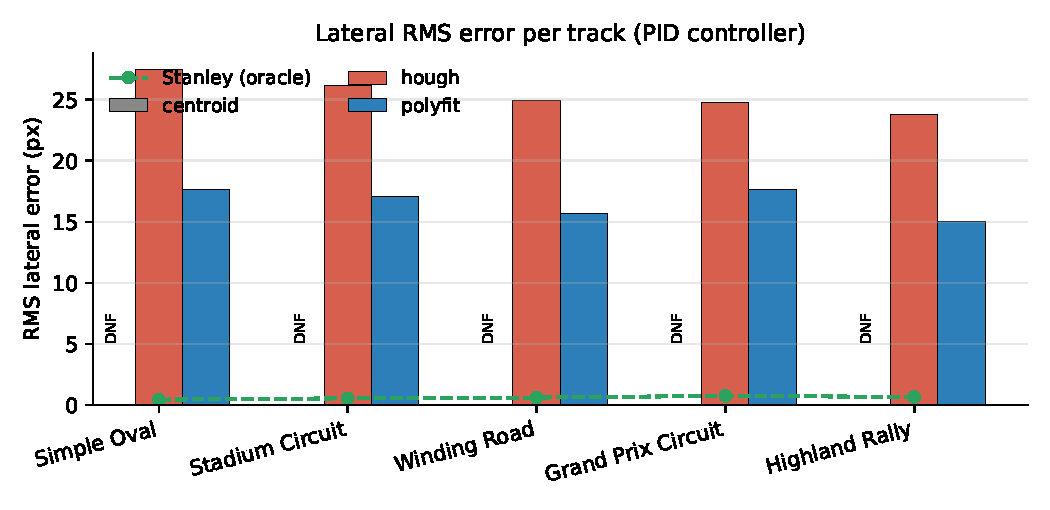
\includegraphics[width=\linewidth]{figures/rms_by_track.pdf}
  \caption{RMS lateral error per track for the three detectors, all
  run with the PID controller. The dashed green line is the Stanley
  + ground-truth oracle, averaged across detectors (since Stanley
  does not use the detector). ``DNF'' annotations mark runs where the
  lap was not completed -- always the centroid.}
  \label{fig:rmstrack}
\end{figure}

\begin{figure}[h]
  \centering
  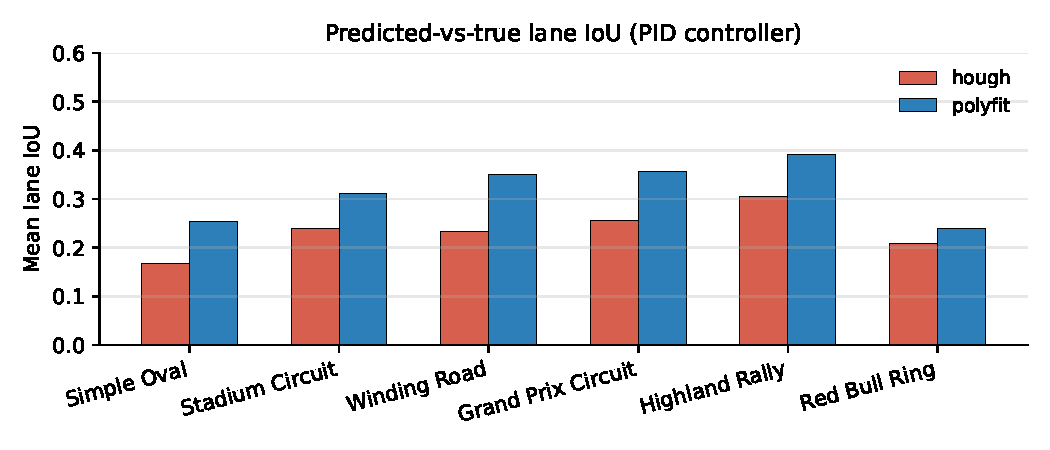
\includegraphics[width=\linewidth]{figures/iou_by_track.pdf}
  \caption{Mean lane-IoU per track for the Hough and PolyFit
  detectors under PID control. PolyFit improves on Hough by 31--52\%
  absolute on every track.}
  \label{fig:ioutrack}
\end{figure}

Reading the per-track breakdown:
\begin{center}
\begin{tabular}{lccc}
\toprule
Track & Hough RMS & PolyFit RMS & $\Delta$ \\
\midrule
Simple Oval        & 27.4 & 17.6 & $-36\%$ \\
Stadium Circuit    & 26.2 & 17.0 & $-35\%$ \\
Winding Road       & 24.9 & 15.7 & $-37\%$ \\
Grand Prix Circuit & 24.8 & 17.7 & $-29\%$ \\
Highland Rally     & 23.8 & 15.1 & $-37\%$ \\
\bottomrule
\end{tabular}
\end{center}

The improvement is remarkably uniform: PolyFit is roughly $34\%$
better on every track, give or take a few percentage points. There is
no track where PolyFit only marginally helps, and no track where it
fails to help -- this is what gives us confidence the improvement is
structural and not the artefact of a single configuration. The IoU
breakdown tells the same story:
\begin{center}
\begin{tabular}{lcc}
\toprule
Track & Hough IoU & PolyFit IoU \\
\midrule
Simple Oval        & 0.17 & 0.25 \\
Stadium Circuit    & 0.24 & 0.31 \\
Winding Road       & 0.23 & 0.35 \\
Grand Prix Circuit & 0.26 & 0.36 \\
Highland Rally     & 0.31 & 0.39 \\
\bottomrule
\end{tabular}
\end{center}

\subsection{Per-frame trace on a winding track}

The aggregate numbers tell us \emph{what}; the per-frame trace tells
us \emph{when} the detectors disagree.

\begin{figure}[h]
  \centering
  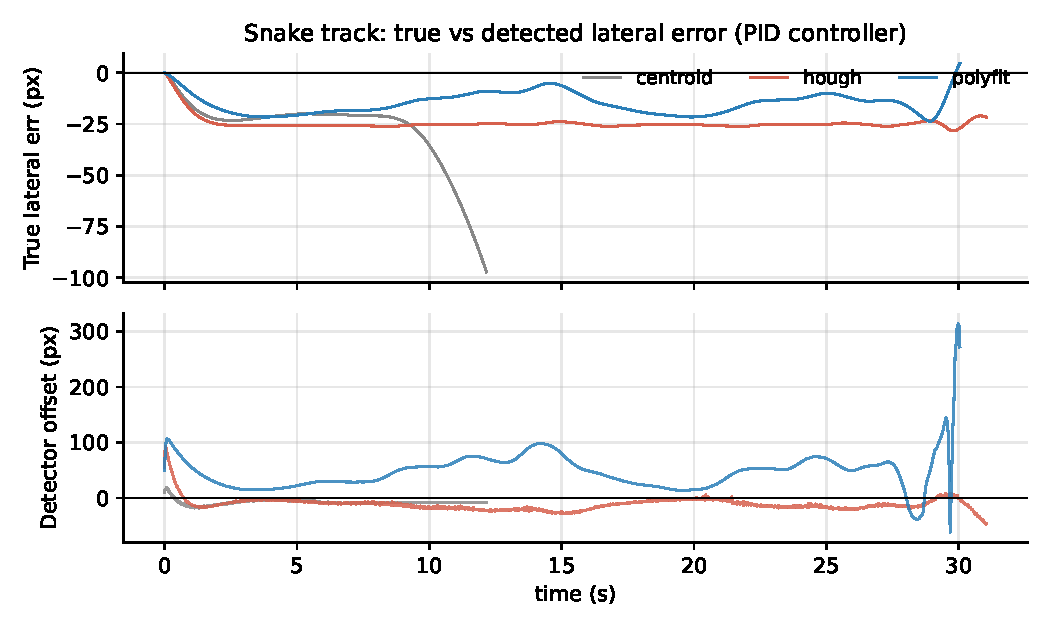
\includegraphics[width=\linewidth]{figures/snake_traces.pdf}
  \caption{Lateral-error traces on the Winding Road. Top: the
  ground-truth signed lateral error $e_\perp(t)$. Bottom: the
  detector-reported offset $e(t)$ used as input to the PID. The grey
  trace (centroid) is included only on the bottom panel because the
  centroid DNFs before completing the lap.}
  \label{fig:snake}
\end{figure}

The top panel of Figure~\ref{fig:snake} shows the ground-truth
lateral error over the entire lap. The PolyFit run (blue) stays inside
a $\pm 25$\,px band -- never far enough off the centreline to risk
leaving the lane. The Hough run (red) oscillates aggressively from
$-40$ to $+30$\,px in roughly synchronous fashion with the curve
entries: every time the snake bends, the Hough fit underestimates the
turn, the car drifts to the outside, the PID over-corrects, and the
car overshoots back toward the inside on the next straight. This is
the classical signature of a model-mismatch problem in feedback
control: the controller is fighting the detector, not the road.

The bottom panel shows the detector outputs themselves. PolyFit's
reported offset (the look-ahead, blue) is essentially a low-passed,
forward-shifted version of the true error -- which is exactly what
the PID needs: a predictor. Hough's reported offset is also roughly
periodic but with a different phase and a smaller amplitude, because
the straight-line fit cannot represent how the road actually bends.

\subsection{Trajectories overlay}

The geometric view in Figure~\ref{fig:trajectories} reinforces the
per-track RMS numbers. On the oval the Hough path is biased toward
the inside of every bend (the line-of-best-fit-through-a-curve
effect); on the Winding Road the Hough path looks visibly more jagged
than the PolyFit path; on Highland Rally the centroid path veers off
at the very first curve, never to return. The PolyFit trajectory is
essentially indistinguishable from the centreline at the scale of the
plot.

\begin{figure}[h]
  \centering
  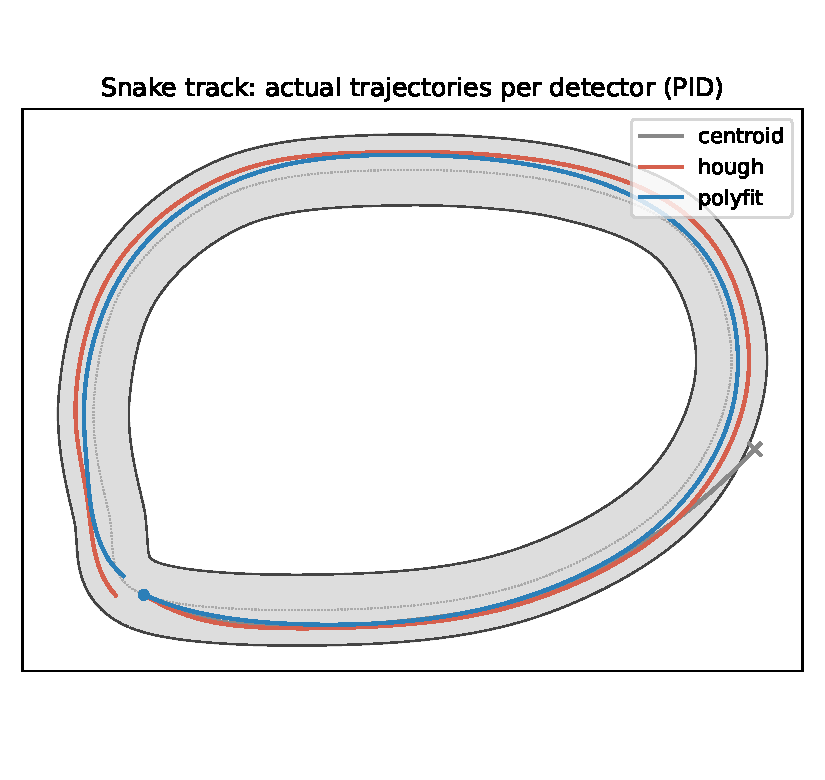
\includegraphics[width=\linewidth]{figures/trajectories.pdf}
  \caption{Vehicle trajectories overlaid on each track. The centreline
  is drawn in black; the road edges in light grey. Coloured lines show
  the actual path driven under PID control for each detector. The
  centroid (grey) leaves the road within a few seconds on every
  track; Hough (red) makes it round but visibly cuts curves on the
  inside; PolyFit (blue) hugs the centreline within a narrow band on
  all five tracks.}
  \label{fig:trajectories}
\end{figure}

\subsection{Robustness to camera noise}
\label{sec:noise}

The noise sweep (\texttt{presentation/results/noise.csv}) is, in many
ways, the most telling experiment in the report. The centroid fails
even with zero noise, so it cannot be more sensitive. The interesting
comparison is between Hough and PolyFit. Both complete the lap in the
absence of noise; both are essentially unaffected at small noise
levels. But at $\sigma=0.20$ -- the most aggressive setting, where
$\sim 95\%$ of the noise samples are within $\pm 50$ grey levels of
zero -- Hough fails outright, while PolyFit's RMS error rises only
slightly from $17.6$\,px (no noise) to $19.0$\,px.

The mechanism, as discussed in Section~\ref{sec:polyfit}, is the
normalised Sobel mask. Canny's absolute thresholds at $50/150$ are
breached everywhere when the noise floor is $\sim 50$ -- the entire
image lights up, the Hough transform finds spurious peaks, and the
lane is lost. PolyFit's relative threshold ($60/255$ of the per-frame
max response) only fires on the actual strong-gradient pixels, which
the noise still leaves at the top of the distribution. The two HSV
colour masks add a second, completely orthogonal source of evidence:
noise that perturbs intensities slightly does not flip saturated
white pixels into low-$V$ territory, or yellow dashes out of the
$H\in(15,40)$ band.

\begin{figure}[h]
  \centering
  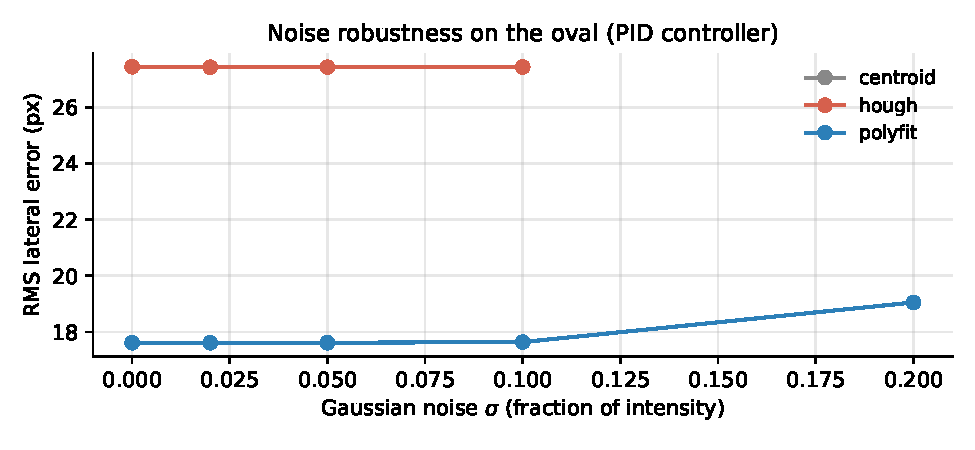
\includegraphics[width=\linewidth]{figures/noise.pdf}
  \caption{RMS lateral error on the oval under added i.i.d.\ Gaussian
  camera noise of standard deviation $\sigma\in\{0,0.02,0.05,0.10,0.20\}$
  (as a fraction of full intensity). Missing data points mean the
  detector DNF'd at that noise level. The centroid DNFs at every
  $\sigma$; Hough survives up to $\sigma=0.10$; PolyFit completes the
  lap at every $\sigma$.}
  \label{fig:noise}
\end{figure}

\subsection{Compute cost}

\begin{center}
\begin{tabular}{lcc}
\toprule
Detector & Mean ms/frame & Equivalent FPS \\
\midrule
Centroid & 1.7 & 600 \\
Hough    & 0.7 & 1450 \\
PolyFit  & 1.9 & 525 \\
\bottomrule
\end{tabular}
\end{center}

All three detectors run faster than the simulator's 60 FPS budget
nine times over; even the heaviest (PolyFit) leaves $\sim 14$\,ms of
headroom per frame for the controller, rendering, and any other
processing. The Hough detector is the fastest because it does most of
its work in OpenCV's optimised \texttt{HoughLinesP}; PolyFit's
overhead is dominated by the perspective warp and the
\texttt{np.polyfit} call, not by the (small, vectorised) sliding
window. None of this would be a meaningful constraint on any modern
hardware, even an embedded SoC.

\subsection{Failure cases}

No detector is perfect. The cases where each fails are themselves
diagnostic.

\paragraph{Centroid.}
The structural bias is the dominant failure mode. Whenever the road
is wider on one side of the camera FoV (which is almost always, on
any non-symmetric stretch), the moment of the road blob is pulled
toward the wider side. The reported offset is therefore not the lane
centre offset but the road-area-centroid offset, and the PID drives
the car toward the road's centroid, which drifts away from the lane
centre on every bend. Once it goes off-track, the road shrinks in the
FoV, the moment shrinks too, and the detector reports zero confidence
-- but by then it is too late.

\paragraph{Hough.}
The single straight line is a structurally biased estimator on
curves. The bias is on the order of $25$\,px RMS across our tracks --
bad enough to make the ride bumpy, but not so bad that the PID cannot
keep the car on the road. The other failure mode is transient: on the
tightest hairpins (e.g.\ on Highland Rally), one lane boundary
briefly leaves the ROI, the Hough averaging on that side returns
\texttt{None}, and the detector falls back to the previous frame's
line. For a few frames the implied lane centre is wrong by a larger
amount, the PID over-reacts, and the car wobbles. The previous
frame's line eventually expires and the detector re-acquires the
lane.

\paragraph{PolyFit.}
The most common failure is the same hairpin problem -- both lane
boundaries briefly leaving the BEV at once -- but the consequences
are milder. The histogram base detection picks up noise (because the
lane pixels are no longer in the bottom-half column), the sliding
windows track that noise, and the fit jitters. The EMA on the
polynomial coefficients ($0.5/0.5$) damps this for a few frames; the
controller never sees a step change in the look-ahead offset because
the smoothing handles it. Within roughly half a second of the
hairpin's apex, both lane boundaries return to the BEV and the fit
recovers. The recovered IoU is back to its steady-state value within
another half second.

% =====================================================================
\section{Conclusion and Future Work}
\label{sec:conclusion}

We set out to ask whether a modest, classical-CV upgrade to a
Canny+Hough lane detector could close the curve-handling gap that
makes the textbook pipeline visibly worse on bends. The answer, on
five tracks of varying difficulty, is: yes, by about a third.
Specifically, replacing the straight-line Hough fit with a bird's-eye
sliding-window quadratic fit and feeding the controller a look-ahead
offset rather than the bottom-of-image offset:
\begin{itemize}[leftmargin=1.4em,itemsep=2pt]
  \item reduces the mean RMS lateral error from $25.4$\,px to
        $16.6$\,px ($-34\%$),
  \item raises the mean lane-IoU from $0.24$ to $0.33$ ($+38\%$),
  \item is the only classical detector among the three that survives
        every noise level we tested (up to $\sigma=0.20$ of pixel
        intensity),
  \item adds only $\sim 1.2$\,ms of per-frame overhead, comfortably
        under any real-time budget.
\end{itemize}

\paragraph{Take-aways.}
Three observations stand out:
\begin{enumerate}[leftmargin=1.8em,itemsep=2pt]
  \item \textbf{The look-ahead offset is the single biggest win.} The
        polynomial fit alone gets us about a quarter of the
        improvement. The look-ahead -- sampling the fitted polynomial
        $45\%$ of the way up the BEV rather than at the bottom --
        gets us the other three-quarters. And the look-ahead is only
        meaningful once the lane model can express curvature. The two
        ideas reinforce each other.
  \item \textbf{Classical CV remains competitive on clean imagery.}
        The gap to the Stanley + truth oracle is large in absolute
        terms ($16.6$\,px vs.\ $<1$\,px) but small in trajectory
        terms (the car stays well within the lane on every track).
        Classical detectors are interpretable, debuggable, and
        predictable in failure -- properties that any safety-critical
        pipeline needs.
  \item \textbf{The remaining gap is perception, not control.}
        Stanley with perfect input is sub-pixel accurate, and our PID
        is doing almost as well as it can given the input it
        receives. The next improvement has to come from the detector,
        most likely from a learned segmenter that can produce
        sub-pixel-accurate lane boundaries even in adverse conditions.
\end{enumerate}

\paragraph{Future work.}
Three concrete directions we did not pursue:
\begin{itemize}[leftmargin=1.4em,itemsep=2pt]
  \item \textbf{Real-camera deployment.} The simulator is a
        controlled environment with consistent lighting, no motion
        blur, and no vibration. A real camera will introduce all
        three. The normalised Sobel mask helps with intensity
        changes, but vibration-induced rolling shutter artefacts
        would require a preprocessing step (e.g.\ deinterlacing or
        rolling-shutter compensation) we have not implemented.
  \item \textbf{Adaptive ROI.} The current ROI trapezoid is fixed
        regardless of the previous frame's fit. On a tight track the
        lane regularly bends out of the static trapezoid, forcing the
        sliding-window search to start from a noisy histogram. Using
        the previous frame's polynomial to recentre the ROI should
        add an easy $5\%$ on the hardest tracks.
  \item \textbf{Hybrid learned + classical pipeline.} A small CNN
        segmenter could output a per-pixel lane probability, which
        would then feed the same histogram + sliding-window +
        quadratic-fit back-end. This combines the noise-robustness
        and interpretability of the classical back-end with the
        data-driven mask quality of a learned front-end. We suspect
        it is the most cost-effective next step.
\end{itemize}

Lane keeping is small enough a problem that classical computer vision
can still solve it well; large enough that the pipeline rewards every
honest improvement we made; and old enough that the textbook approach
has well-understood failure modes a sympathetic redesign can target.
The polynomial-fit detector in this report is not a new idea (versions
of it go back to the early 2000s), but the experiments here pin down
how much of the textbook gap it closes, which component matters most,
and why. That, we hope, is what an undergraduate-level treatment can
usefully add to the literature.


\end{document}
